\documentclass[a4paper, 12pt, oneside]{report}

\usepackage[utf8]{inputenc}
\usepackage{lmodern}
\usepackage{layout}
\usepackage{emptypage}
\usepackage{fancyhdr}
%\usepackage[Conny]{fncychap}
%\usepackage{graphicx}
\usepackage{subfigure} % subfiguras
\usepackage{caption}
\usepackage{mathtools}
\usepackage{hyperref}
\usepackage[a4paper,top=3cm, bottom=3cm, inner=2.5cm, outer=2.5cm]{geometry}
\usepackage{listings}
\usepackage[spanish]{babel}
\usepackage{url}
\usepackage{float}
\usepackage{multirow}
\usepackage{rotating} 
\usepackage{color}
\usepackage{colortbl}
\usepackage[table]{xcolor}
\usepackage[spanish]{babel}


\usepackage[acronym, nonumberlist]{glossaries}
\makeglossaries
\chapter*{Acrónimos}

\acrodef{MNIST}{Modified National Institute of Standards and Technology}
\acrodef{NIST}{National Institute of Standards and Technology}
\acrodef{ReLU}{Rectified Linear Unit}
\acrodef{COCO}{Common Objects in Context}
\acrodef{JSON}{JavaScript Object Notation}
\acrodef{RLE}{Run-Length Encoding}
\acrodef{VOC}{Visual Objects Classes}


\makeatletter
\renewcommand{\@makeschapterhead}[1]{%
%  \vspace*{50\p@}%
  \vspace*{0\p@}%
  {\parindent \z@ \raggedright
    \normalfont
    \interlinepenalty\@M
    \Huge \bfseries  #1\par \nobreak
%    \vskip 40\p@
    \vskip 15\p@
  }}
\makeatother

\renewcommand{\baselinestretch}{1.4}
\setlength{\headheight}{16pt} 
\captionsetup{justification=justified}
\pretolerance=1000

\chead[]{}
\rhead[]{}
\renewcommand{\headrulewidth}{0.5pt}

\pagestyle{empty}

\title{Deep-learning para detección de vehículos}
\author{Nuria Oyaga de Frutos}

\lstset{
	float=hbp,
	basicstyle=\ttfamily\small,
	columns=flexible,
	tabsize=4,
	frame=single,
	extendedchars=true,
	showspaces=false,
	showstringspaces=false,
	numbers=none,
	numberstyle=\tiny,
	breaklines=false,
	breakautoindent=true,
	captionpos=b
}
\setcounter{tocdepth}{4}
\setcounter{secnumdepth}{4}

\definecolor{lightgray}{gray}{0.9}

\begin{document}
%%%%%%%%%%%%%%% Portada %%%%%%%%%%%%%%%%%%%%
\begin{titlepage}
	
	\begin{center}
		\vspace*{7.7mm}
		\begin{center}
			
\includegraphics[width=0.4\linewidth]{figures/logo.jpg}
		\end{center}
		\vspace{6.5mm}
		
		\fontsize{15.5}{14}\selectfont ESCUELA TÉCNICA SUPERIOR DE INGENIERÍA DE TELECOMUNICACIÓN
		\vspace{13mm}
		
		\fontsize{14}{14}\selectfont GRADO EN INGENIERÍA EN SISTEMAS \\ AUDIOVISUALES Y MULTIMEDIA
		
		\vspace{70pt}
		
		\fontfamily{lmss}\fontsize{15.7}{14}\selectfont \textbf{TRABAJO FIN DE GRADO} 
		
		\vspace{25mm}
		\begin{huge}
			Análisis de Aprendizaje Profundo com\\ la plataforma Caffe
		\end{huge}
		
		\vspace{25mm}
		
		\begin{large}
			Autor: Nuria Oyaga de Frutos
			
			Tutor: Inmaculada Mora Jiménez
			
			Cotutor: José María Cañas Plaza
			
			\vspace{10mm}
		\end{large}
		\begin{normalsize}
			Curso académico 2016/2017		
		\end{normalsize}
		\vspace{10mm}
		
	\end{center}
	
\end{titlepage}

\pagebreak
\thispagestyle{empty}
\vspace*{12cm}

\begin{flushright}


\includegraphics[height=1.0cm]{figures/CC-BY-SA.png}

\vspace*{0.5cm}

\copyright 2017 Nuria Oyaga de Frutos

\vspace*{0.3cm}

Esta obra está distribuida bajo la licencia de 

``Reconocimiento-CompartirIgual 4.0 Internacional (CC BY-SA 4.0)''

de Creative Commons.

\vspace{0.2cm}

Para ver una copia de esta licencia, visite

http://creativecommons.org/licenses/by-sa/4.0/ o envíe

una carta a Creative Commons, 171 Second Street, Suite 300,

San Francisco, California 94105, USA.

\end{flushright}

\pagenumbering{Roman}

%%%%%%%%%%%%%%% Agradecimientos %%%%%%%%%%%%
\chapter*{Agradecimientos}


%%%%%%%%%%%%%%% Resumen %%%%%%%%%%%%%%%%%%%%
\chapter*{Resumen}

En los últimos años, la investigación para conseguir que las máquinas perciban escenas y estímulos visuales con la robustez y rapidez que lo hacen los humanos, ha sido altamente desarrollada. En este aspecto, el campo de la Inteligencia Artificial, y en concreto nuevos esquemas de aprendizaje máquina como el aprendizaje profundo (\textit{Deep Learning}) con redes neuronales convolucionales, han experimentado un claro avance, permitiendo por ejemplo la identificación robusta de personas o la detección fiable de vehículos. A diferencia de otros, este aprendizaje no requiere de una etapa externa de extracción de características, pues la extracción se realiza en la propia red. Este trabajo analiza las redes neuronales convolucionales mediante el uso de la plataforma Caffe, que permite el entrenamiento de estas redes y facilita la implementación en aplicaciones propias.\\

En visión artificial, las redes neuronales pueden ser utilizadas para la resolución de dos problemas. Por un lado, pueden clasificar el contenido de una imagen en una categoría de entre un conjunto de clases indicadas durante el aprendizaje. Por otro lado, pueden detectar estímulos dentro de la imagen, obteniendo como salida un conjunto de cajas delimitadoras que indiquen la presencia de determinados estímulos.\\

En este trabajo se ha construido un componente en Python que clasifica números manuscritos utilizando una red neuronal de Caffe. También se ha estudiado el efecto que entrenar la red con diferentes bases de datos tiene sobre las prestaciones del clasificador. Se ha utilizado la base de datos MNIST, compuesta por imágenes de dígitos manuscritos. A esta base de datos se le ha aplicado un preprocesamiento para lograr una red más robusta. En concreto, se han considerado transformaciones de escalado, rotación, traslación y contaminación con ruido aditivo. Posteriormente, se ha aplicado un filtro de bordes de Sobel para diseñar una red que premita resolver el problema independientemente de la procedencia de las imágenes (base de datos MNIST, imágenes captadas con una cámara). Adicionalmente, tambien se ha explorado la detección de estímulos interesantes con redes neuronales de Caffe.


%%%%%%%%%%%%%%% Índices %%%%%%%%%%%%%%%%%%%%
\renewcommand{\tablename}{Tabla}
\renewcommand{\listtablename}{Índice de tablas}
\tableofcontents

\cleardoublepage % Í­ndice de figuras
\addcontentsline{toc}{chapter}{\listfigurename}
\listoffigures

\cleardoublepage % Í­ndice de tablas
\addcontentsline{toc}{chapter}{Índice de tablas}
\listoftables 


%%%%%%%%%%%%%%% Acronimos %%%%%%%%%%%%%%%%%%%%
\renewcommand{\acronymname}{Acrónimos}
\cleardoublepage
\addcontentsline{toc}{chapter}{Acrónimos}
\printglossary[type=\acronymtype]

\cleardoublepage
%%%%%%%%%%%%%%% Capí­tulos %%%%%%%%%%%%%%%%%%
\pagestyle{fancy}
\pagenumbering{arabic}
\setlength{\parindent}{6mm}

\lhead[]{CAPÍTULO \thechapter. INTRODUCCIÓN}
\chapter{Introducción y objetivos}\label{cap.introduccion}
El objetivo general de este trabajo se sitúa en  entender el funcionamiento del aprendizaje profundo con redes neuronales, utilizando para ello una de las plataformas existentes para el desarrollo de las mismas, Caffe.\\

En este capítulo se situará el trabajo en el marco existente en la actualidad, explicando de manera genérica en qué consiste el aprendizaje profundo, el por qué del uso de una determinada plataforma y los problemas que es posible abordar con esta técnica. Además, se expondrán los objetivos concretos de este proyecto, la metodología empleada para alcanzarlos y un pequeño resumen de cómo se ha estructurado el trabajo.

\section{Contexto y motivación}

Desde que los primeros ordenadores fueron programados, el ser humano se ha planteado la posibilidad de conseguir que estas máquinas adquieran inteligencia, logrando que realicen tareas propias de las personas. Ejemplos de estas tareas son automatizar el trabajo de rutina, entender el habla o las imágenes, hacer diagnósticos en medicina y apoyar la investigación científica básica. Hoy en día, la \acrfull{ia}~\cite{Goodfellow-et-al-2016}, como se denomina al campo que desarrolla estas tareas, cada vez adquiere más presencia, con un alto potencial por sus muchas aplicaciones prácticas y temas de investigación activos.\\

En los orígenes de la \acrshort{ia} se abordaron y resolvieron problemas que no son de resolución inmediata para los seres humanos, pero relativamente sencillos para los ordenadores, problemas que pueden describirse mediante una lista de reglas formales. Una meta actual, aún más ambiciosa, consiste en resolver tareas que son fáciles de realizar para las personas pero difíciles de describir formalmente.Se trata de problemas que son resueltos de manera rápida e intuitiva por el ser humano como, por ejemplo, el reconocimiento visual de las personas.\\

La \acrshort{ia} abarca varios campos y en este trabajo el foco estará puesto sobre la \acrfull{va}. La \acrshort{va} trata de analizar y procesar imágenes del mundo real de tal manera que un ordenador pueda establecer conclusiones sobre las mismas. La idea básica es tratar de trasladar a una máquina la forma en que el ser usa sus ojos y su cerebro para comprender el mundo que le rodea, permitiendo a las mismas tomar decisiones y actuar según la situación. Para lograr el aprendizaje de las máquinas es necesario aplicar conocimientos de distintos campos como la geometría, la estadística, la física y otras disciplinas.\\

Para conseguir materializar el concepto de la \acrshort{va} se hace uso de las Redes Neuronales Artificiales (RNA). Estas redes están compuestas por capas de neuronas interconectadas que tratan de imitar el comportamiento de las mismas en el cerebro del ser humano. La neurona biológica, consta de un cuerpo celular (soma) del que surge un denso árbol de ramificaciones (dendritas) y una fibra tubular (axón). Esta estructura se asemeja a un procesador de información simple formado por un canal de entrada, similar a las dentritas, un procesador, cuya función se asemeja a la del soma, y un canal de salida, equiparable al axón~\cite{rna}. Además, entre las neuronas biológicas se establecen una serie de conexiones unidireccionales, conocidas como sinapsis, que son emuladas en el sistema artificial por el conjunto de pesos. En la Figura~\ref{fig.rna} se muestra la similitud entre ambos tipos de neuronas. Una vez entendida la unidad de proceso, se puede definir una \acrshort{rna} como la conexión de este elemento de diferentes formas, dando lugar a diferentes tipos de redes. Para este trabajo tiene interés la red multicapa, que se compone de dos o más capas de neuronas que están conectadas entre ellas, realizando un procesado no lineal de los datos que se presentan a la entrada.\\

\begin{figure}[H]
	\begin{center}
		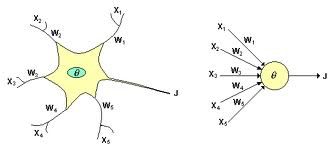
\includegraphics[width=0.7\textwidth]{figures/rna.jpg}
		\caption{Comparación de neurona artificial (derecha) y biológica (izquierda). Imagen obtenida de~\cite{rna}.}
		\label{fig.rna}
	\end{center}
\end{figure}

Tras definir el contexto general, este trabajo se centra en el Aprendizaje Profundo, situado dentro del marco de la IA, que permite obtener el conocimiento entrenando a las máquinas con ejemplos, sin necesidad de realizar una extracción de características previa, sino que es la propia red que se obtiene la encargada de ello. En la Figura~\ref{fig.aprendizaje}, se sitúa esta solución en el marco de la \acrshort{ia} y sus diferentes divisiones.

\begin{figure}[H]
	\begin{center}
		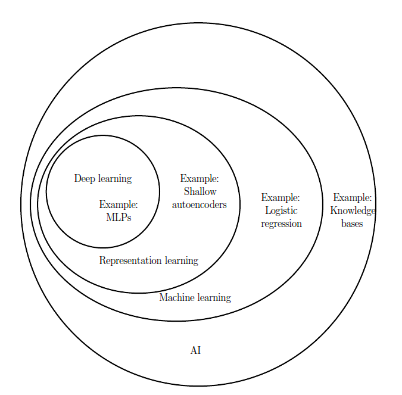
\includegraphics[width=0.6\textwidth]{figures/aprendizaje}
		\caption{Diagrama de Venn que muestra el marco de la \acrshort{ia}. Imagen obtenida de~\cite{Goodfellow-et-al-2016}.}
		\label{fig.aprendizaje}
	\end{center}
\end{figure}

En términos generales, la \acrshort{ia} contiene al Aprendizaje Máquina (\textit{Machine Learning}) definido como la capacidad de las computadoras para adquirir sus propios conocimientos, extrayendo patrones de datos sin procesar. A su vez, en el interior de la misma se sitúa el Aprendizaje de la Representación (\textit{Representation Learning}), que utiliza el aprendizaje máquina para descubrir, no sólo el mapeo de la representación a la salida, sino también la representación misma. Finalmente, en este último bloque estaría situado el Aprendizaje Profundo (\textit{Deep~Learning}), que permite a la computadora construir conceptos complejos a partir de conceptos más sencillos.\\

Dentro del Aprendizaje Profundo es posible aplicar diversas técnicas. La técnica más común y la que será empleada en este trabajo son las \acrfull{cnn}, que pretenden simular el funcionamiento del cerebro humano para establecer conclusiones sobre los datos introducidos a la misma utilizando filtros convolucionales.  La propiedad más importante del aprendizaje con redes neuronales es la capacidad de generalización, que será estimada gracias a una base de datos específica, denominada de test. Se trata de la capacidad que tiene una red de identificar una muestra que no era conocida para ella.\\

Las \acrshort{cnn} tienen una estructura especial, mostrada en la Figura~\ref{fig.cnn}. Está compuesta, generalmente, por una capa convolucional, que implementa una operación de convolución, y una capa de submuestreo o agrupación, que genera características invariantes calculando estadísticas de las activaciones de convolución a partir de un pequeño campo receptivo. Cada neurona en una capa oculta se conectará a un pequeño campo de la capa anterior, denominado campo receptivo local. En las \acrshort{cnn}, las neuronas están organizadas en múltiples capas ocultas paralelas, denominadas mapas de características, de tal manera que cada neurona en un mapa de características está conectada a un campo receptivo local. Para cada mapa de características, todas las neuronas comparten el mismo parámetro de peso que se conoce como filtro o \textit{kernel}~\cite{cnn}.

\begin{figure}[H]
	\begin{center}
		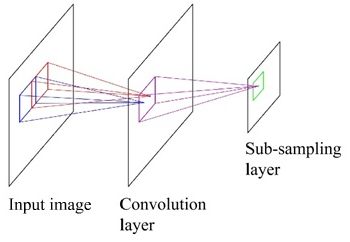
\includegraphics[width=0.4\textwidth]{figures/cnn}
		\caption{Estructura de \acrshort{cnn}. Imagen obtenida de~\cite{cnn}.}
		\label{fig.cnn}
	\end{center}
\end{figure}

En la actualidad existen múltiples disciplinas que tratan de incluir esta tecnología en su ámbito de trabajo para obtener resultados de forma más rápida y precisa. Una de las disciplinas que mas esfuerzos pone en la investigación de este campo es la medicina, cuyo principal objetivo es lograr diagnosticar y tratar, e incluso prevenir enfermedades como el cáncer. Un ejemplo de ello fue llevado a cabo por el \textit{\acrfull{bidmc}} y la Escuela de Medicina de Harvard, que consiguió el premio máximo en dos categorías del \acrfull{isbi} para la detección del cáncer de mama. El equipo, utilizando la plataforma Caffe, comenzó entrenando su máquina con cientos de diapositivas marcadas para indicar qué partes tienen células cancerosas y cuáles normales, identificando qué tipo de diapositivas eran más complicadas y alimentando el sistema con muestras más difíciles. Con este método, se obtuvo un acierto 92 por ciento y, aunque todavía no compite con los patólogos humanos, cuya precisión es el 96 por ciento, se obtiene un gran avance en este campo~\cite{2016arXiv160605718W}.\\

\begin{figure}[H]
	\begin{center}
		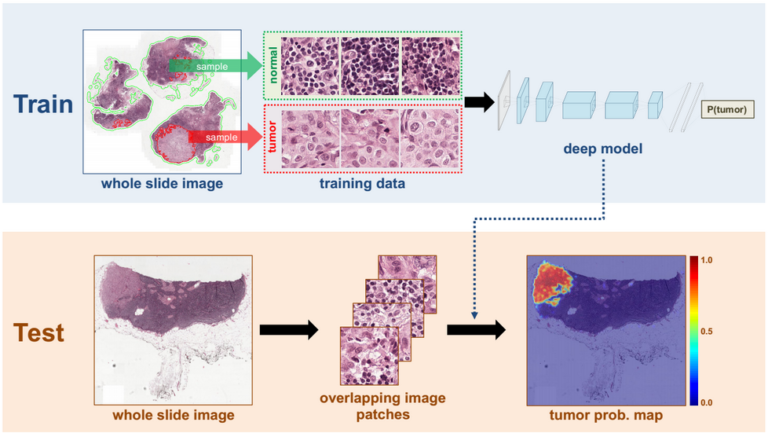
\includegraphics[width=0.6\textwidth]{figures/cancer}
		\caption{Marco utilizado para la detección del cáncer de mama. Imagen obtenida de~\cite{2016arXiv160605718W}.}
	\end{center}
\end{figure}

Un segundo ejemplo que está a la orden del día es la aplicación en la conducción autónoma. La idea de que un coche pueda manejarse en la carretera por sí mismo, sin necesidad de la existencia de un conductor que realice el trabajo, es tan llamativa que existen múltiples organizaciones que tratan de abarcar este problema. Existen tres paradigmas, mostrados en la Figura~\ref{fig.conduccion}, que permiten abarcar el problema de la conducción autónoma: (1)~el enfoque de percepción mediada, que analiza una escena entera para tomar una decisión de conducción; (2)~el enfoque de reflejo de comportamiento, que directamente mapea una imagen de entrada a una acción de conducción por un regresor; y (3)~el enfoque basado en la percepción directa para estimar la posibilidad para conducir. Este último fue desarrollado por la Universidad de Princeton se propone mapear una imagen de entrada a un pequeño número de indicadores de percepción clave, que se relacionan directamente con la disponibilidad de un estado de carretera o tráfico para la conducción. Esta representación proporciona un conjunto de descripciones compactas pero completas de la escena, permitiendo a un controlador conducir de forma autónoma.

\begin{figure}[H]
	\begin{center}
		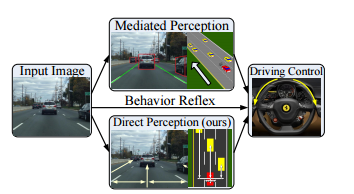
\includegraphics[width=0.6\textwidth]{figures/conduccion}
		\caption{Paradigmas de la conducción autónoma. Imagen obtenida de~\cite{2015arXiv150500256C}.}
		\label{fig.conduccion}
	\end{center}
\end{figure}

Otro ejemplo de aplicación es la traducción automática que, a pesar de haber existido durante mucho tiempo, el aprendizaje profundo consigue los mejores resultados en la traducción automática de texto e imágenes. Gracias a las \acrshort{cnn} es posible identificar las imágenes que tienen letras y dónde se situan éstas en la escena. Una vez identificadas, pueden convertirse en texto, traducirlo y recrear la imagen con esa traducción. Esta técnica es conocida como traducción visual instantánea~\cite{traduccion}.

\begin{figure}[H]
	\begin{center}
		
\includegraphics[width=0.6\textwidth]{figures/traduccion}
		\caption{Ejemplo de traducción visual instantánea. Imagen obtenida de~\cite{traduccion}.}
	\end{center}
\end{figure}

Un último ejemplo de aplicación de esta tecnología se basa en adición automática de sonidos a películas mudas, donde el sistema debe sintetizar sonidos para que coincidan con un vídeo silencioso. Para esta tarea el sistema se entrena utilizando 1000 ejemplos de vídeo con el sonido de un tambor golpeando diferentes superficies y creando diferentes sonidos. El modelo de aprendizaje profundo asocia los fotogramas de vídeo con una base de datos de sonidos pre-grabados para seleccionar el sonido que mejor se adapte a lo que está sucediendo en la escena y lo reproduzca~\cite{2015arXiv151208512O}.

\begin{figure}[H]
	\begin{center}
		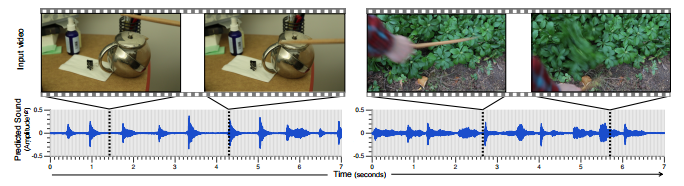
\includegraphics[width=0.8\textwidth]{figures/sonido}
		\caption{Ejemplo adición de sonidos a películas mudas. Imagen obtenida de~\cite{2015arXiv151208512O}.}
	\end{center}
\end{figure}


Además de las aplicaciones explicadas anteriormente existen muchísimas otras que surgen de las propias inquietudes del ser humano: reconocimiento facial, videovigilancia, identificación de posiciones... Sin embargo, ninguna de ellas ha sido desarrollada por completo, dejando una gran vía de investigación sobre el tema.\\

Este trabajo se centrará en la clasificación y detección de imágenes estáticas o en movimiento. La diferencia entre ambas aplicaciones es que la detección permite identificar en una única imagen diferentes objetos, independientemente del tamaño y la posición en la que se encuentren, mientras que la clasificación identifica una imagen entrante a la red como perteneciente a una clase determinada.\\

Por último, para implementar lo explicado anteriormente existen múltiples plataformas que facilitan el entrenamiento y la implementación de estas redes. TensorFlow, Keras, Theano, Caffe, Lassagne o Torch son algunos de los ejemplos más conocidos de estas plataformas. En este trabajo se utilizará la plataforma Caffe, una de las más veteranas. La elección de esta plataforma radica en el gran número de modelos pre-entrenados que proporciona la misma para poder implementar en las aplicaciones ahorrando tiempo al nuevo desarrollador. Además está centrado en la \acrshort{va}, lugar hacia el que se enfoca este trabajo, y, en caso de querer entrenar una nuevo red, resulta bastante rápido.\\


\section{Objetivos} \label{sec.objetivos}
Una vez contextualizado en trabajo, el objetivo general es claro: se pretende ahondar en el mundo de la \acrshort{ia}, en concreto en técnicas de Aprendizaje Profundo y \acrshort{cnn}, para obtener resultados que puedan resultar interesantes y desarrollar una aplicación que permita implementar estas técnicas con la mayor exactitud posible. Este objetivo general ha sido  articulado en varios subobjetivos concretos: 

\begin{itemize}
	\item \textbf{Estudio de la plataforma Caffe.} Se pretende estudiar la plataforma escogida para un correcto uso de la misma y la obtención de las redes que sean necesarias.
	\item \textbf{Desarrollo de componente que permita la clasificación de dígitos}, integrando una red entrenada con Caffe en el mismo.
	\item \textbf{Desarrollo de un banco de pruebas}, que permita agilizar la obtención de parámetros de evaluación de las distintas redes entrenadas.
	\item \textbf{Estudio y mejora de redes neuronales para la clasificación de dígitos.} Se realizarán diversas pruebas para tratar de alcanzar la red más robusta posible y utilizarla en el componente desarrollado.
	\item \textbf{Primera aproximación a la detección de Caffe.} Se estudiará la detección \acrfull{ssd} con Caffe para estímulos interesantes para aplicaciones futuras como personas, coches, bicicletas o señales de tráfico.
\end{itemize}

En la Figura~\ref{fig.diagrama} se desglosa, por semanas, el tiempo que ha llevado cada una de las tareas para la consecución de los objetivos.

\begin{figure}[H]
	\begin{center}
		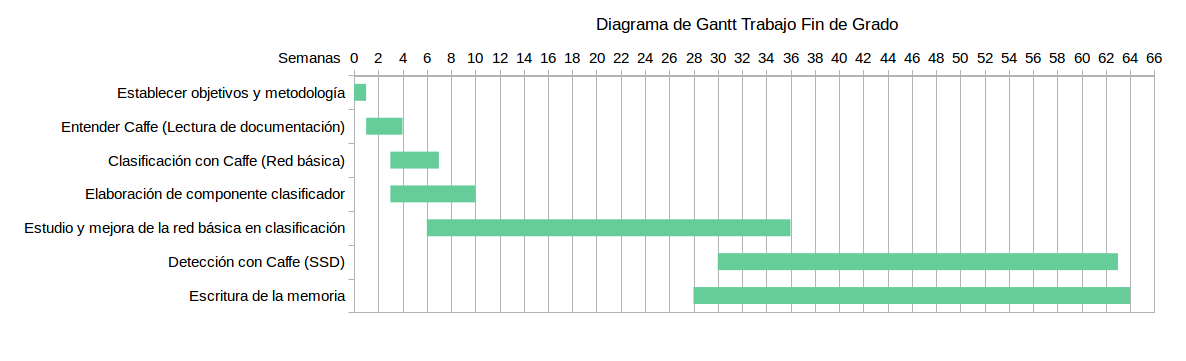
\includegraphics[width=1\textwidth]{figures/diagrama}
		\caption{Diagrama de Gantt del trabajo realizado.}
		\label{fig.diagrama}
	\end{center}
\end{figure}

\section{Metodología}
Para la consecución de los objetivos marcados se han utilizado varias herramientas que han permitido el seguimiento del trabajo por todos los miembros del grupo, permitiendo a todos ellos estar al tanto del trabajo realizado y aportar los comentarios o correcciones que se consideren necesarias.\\

Como herramienta principal, se establecieron reuniones semanales con todos los miembros del grupo, José María Cañas, Inmaculada Mora y David Pascual, que permitieron poner en común y discutir los resultados obtenidos y acordar las vías a seguir durante la siguiente semana.\\

Como herramientas complementarias, se utilizó una bitácora y un repositorio de Git Hub, que permitieron agilizar las reuniones al tener acceso de antemano al trabajo realizado. La bitácora se desarrolló empleando la \textit{Wiki} de JdeRobot\footnote{http://jderobot.org/Noyaga-tfg}, redactando cada semana el trabajo realizado y los resultados obtenidos. El repositorio de Git Hub\footnote{https://github.com/RoboticsURJC-students/2016-tfg-nuria-oyaga} permitió a todos los miembros del grupo acceder al código desarrollado, probarlo y establecer correcciones sobre el mismo.\\

El enfoque de desarrollo que se ha llevado a cabo es similiar al enfoque en espiral. Se establecen cuatro fases principales que son recorridas en forma de caracola. En primer lugar se marcaron los objetivos a alcanzar, seguido de una fase de análisis de riesgo para evaluar qué problemas era posible encontrarse al empezar el desarrollo. Tras evaluar las amenazas se procedió al propio desarrollo del trabajo y una última fase de evaluación del resultado obtenido. No existe un número fijo de iteraciones, produciéndose tantas como sean necesarias para obtener un resultado adecuado, incrementando en cada iteración el alcance del trabajo.

\section{Estructura de la memoria}
Para mostrar el trabajo realizado y los objetivos conseguidos se elabora la memoria con la estructura mostrada a continuación.\\

En el \textbf{Capítulo 1, Introducción y objetivos,} se sitúa el trabajo en el marco actual de la tecnología, la \acrshort{ia} y la sociedad en general. A continuación se establecen las metas que se pretenden alcanzar con el mismo.\\

El \textbf{Capítulo 2, Infraestructura,} describe todo el \textit{software} utilizado en el proyecto, incluyendo la principal plataforma, Caffe, y los conjuntos de datos empleados para la obtención y evaluación de las redes neuronales. Además, se explican los diferentes parámetros que serán empleados para evaluar las prestaciones de las redes creadas.\\

En el \textbf{Capítulo 3, Clasificación con Aprendizaje Profundo,} se expone todo el trabajo realizado para abordar el problema de la clasificación de dígitos con \acrshort{cnn}. En concreto, se describe el funcionamiento de Caffe en la clasificación, el componente creado, y las pruebas realizadas para conseguir una red robusta, con sus correspondientes resultados.\\

En el \textbf{Capítulo 4, Detección con Aprendizaje Profundo,}  se proporciona la información necesaria para realizar la detección con Caffe. Se muestran algunos resultados de pruebas preliminares, realizadas para una mejor comprensión del proceso de detección.\\

Por útlimo, el \textbf{Capítulo 5, Conclusiones y líneas futuras,} resume las conclusiones obtenidas en el trabajo y establece un posible plan de actuación futuro para continuar con la investigación en el tema que se aborda en el trabajo.

\lhead[]{CAPÍTULO \thechapter. INFRAESTRUCTURA}
\chapter{Infraestructura}\label{cap.infraestructura}
En este capítulo se expondrán los principales componentes software utilizados, centrados, principalmente, en la conexión con la cámara y el desarrollo, entrenamiento y test de la red neuronal. Además, se expone una descripción de las bases de datos de las que se partirá para realizar las distintas pruebas sobre la red neuronal. Estas bases de datos serán luego modificadas y adaptadas para el problema concreto que se plantee, permitiendo obtener diversas conclusiones acerca del comportamiento de la propia red y, así, emplear la más adecuada. Por último, serán expuestas los parámetros empleados para evaluar el impacto del aprendizaje en las redes neuronales y que permitirán escoger la red más adecuada para el problema.\\

\section{Software}

\subsection{JdeRobot}\label{sec.jderobot}
JdeRobot~\footnote{http://jderobot.org} es una plataforma de software libre que facilita la tarea de los desarrolladores en el campo de la robótica, visión por computador y otras relacionadas, siendo este su principal fin.\\ 

Está escrito en su mayoría en el lenguaje C ++ y proporciona un entorno de programación basado en componentes distribuidas, de tal manera que una aplicación está formada por una colección de varios componentes asincrónos y concurrentes. Esta estructura permite la ejecución de los distintos componentes en diferentes equipos, estableciendo una conexión entre ellos mediante el middleware de comunicaciones ICE. Además, se obtiene gran flexibiidad a la hora de desarrollar las aplicaciones, ya que estos componentes pueden escribirse en C ++, Python, Java, etc. y todos ellos interactúan a través de interfaces ICE explícitas.\\ 

A pesar de que esta plataforma incluye una gran variedad de herramientas y librerías para la programación de robots, y de una amplia gama de componentes previamente desarrollados para realizar tareas comunes en este ámbito, su uso no es la verdadera finalidad del proyecto, ya que únicamente se centrará en la utilización de uno de sus componentes para facilitar la obtención de las imágenes.
\vspace{10pt}
\begin{description}
\item[Camera Server] \hfill 
\vspace{10pt}
\\
Se trata de un componente que permite servir a un número determinado de cámaras, ya sean reales o simuladas, a partir de un archivo de vídeo. Internamente utiliza \textit{gstreamer} para el manejo y el procesamiento de las diferentes fuentes de vídeo.\\
\vspace{-10pt}
\\
Para su uso, es necesario editar su fichero de configuración, adaptándolo a las necesidades concretas que plantee la máquina. Dentro de este fichero se permite especificar los siguientes campos:\\
\vspace{-20pt}
\begin{itemize}
    \item Configuración de la red, donde se indica la dirección del servidor que va a recibir la petición.
    \item Número de cámaras que se servirán.
    \item Configuración de las cámaras. Se podrán modificar los siguientes campos para cada cámara:
    \begin{itemize}
         \item Nombre y breve descripción
         \item URI: string que define la fuente de vídeo
     	 \item Numerador y denominador del frame rate
         \item Altura y anchura de la imagen
         \item Formato de la imagen
         \item Invertir o no la imagen 
    \end{itemize}
\end{itemize}
\end{description}

\subsection{Caffe}\label{sec.caffe}
Caffe~\cite{jia2014caffe} es una plataforma de aprendizaje profundo que permite el desarrollo, entrenamiento y evaluación de redes neuronales. Incluye, además, modelos y ejemplos previamente trabajados para un mejor entendimiento de las redes neuronales. Es una plataforma de software libre, escrito en C ++, que utiliza la librería CUDA para el aprendizaje profundo y permite interfaces escritas en Python o Matlab.\\ 

Esta plataforma es interesante por múltiples factores. Además de incluir diferentes ejemplos y modelos ya entrenados, lo que ofrece mayor agilidad a la hora de empezar a entender el funcionamiento de las redes neuronales, es destacable la velocidad que ésta ofrece para el entrenamiento de las redes y su posterior evaluación, ya que está prevista con varios indicadores que permiten evaluar la propia red y compararla con otras.\\ 

Su base se encuentra en las redes neuronales convolucionales explicadas en el Capítulo \ref{cap.introduccion}, utilizando un entrenamiento por lotes. En concreto, su estructura y funcionamiento básico queda explicado en la Figura~\ref{fig.redCaffe}.\\

\begin{figure}[H]
	\begin{center}
		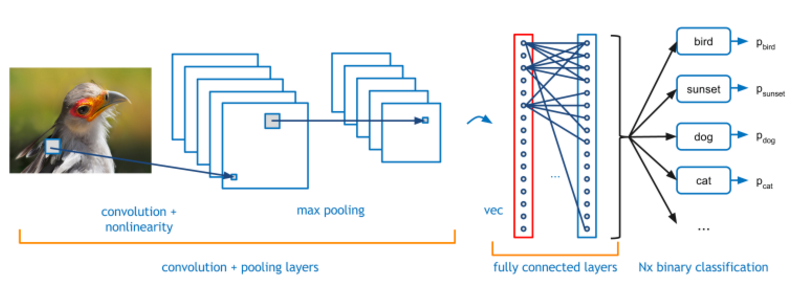
\includegraphics[width=0.6\textwidth]{figures/red_caffe}
		\caption{Estructura y funcionamiento básico de red en Caffe. Figura obtenida de~\cite{caffe}}
		\label{fig.redCaffe}
	\end{center}
\end{figure}

La plataforma utiliza una serie de capas (\textit{layers}), que, según su configuración y la distinta conexión entre ellas, permite la creación de diferentes redes neuronales. Estas capas se dividen en varios grupos, en función del tipo de entrada, el tipo de salida o la función que realiza cada una de ellas. Este trabajo no utiliza todas las capas existentes en la plataforma, a continuación se explicarán cada una de las capas empleadas, clasificadas según al grupo que pertenecen.
\vspace{20pt}
\begin{description}
\item[\textit{Data Layers}] \hfill 
\vspace{10pt}
\\
	Su uso se centra en la introducción de datos a la red neuronal, y estarán situadas siempre en la parte inferior de la misma. Estos datos provienen de diferentes vías que pueden ser: bases de datos eficientes como LMDB, utilizada en este trabajo, diréctamente desde la memoria o desde archivos en disco en HDF5 o formatos de imagen comunes.\\
	\vspace{-10pt}
	\\
	Dentro de esta capa es posible, además de especificar la ruta de los datos y el tamaño del lote (\textit{batch}), indicar la fase en la que se utilizarán los datos, entrenamiento o evaluación, así como algunos parámetros de transformación para el preprocesamiento de la imagen. En concreto, en este trabajo, se utilizarán datos de entrada para ambas fases y un factor de escala para establecer el rango de las imágenes en [0,1].
	\vspace{15pt}
	
\item[\textit{Vision Layers}] \hfill 
\vspace{10pt}
\\
	Este tipo de capas, típicamente toman una imagen de entrada y producen otra de salida, de forma que, aplicando una operación particular a alguna región de la entrada, se obtiene la región correspondiente de la salida. Caffe dispone de varias capas de este estilo, a continuación se comentan las dos utilizadas en el trabajo.
	\vspace{10pt}
	\begin{description}
	\item[\textit{Convolution Layer}] \hfill 
	\vspace{5pt}
	\\
		Realiza la convolución de la imagen de entrada con un conjunto de filtros de aprendizaje, cada uno produciendo un mapa de características en la imagen de salida. Se deben especificar datos como el número de salidas, el tamaño del filtro, el desplazamiento entre cada paso del filtro, y la inicialización y relleno de los pesos y \textit{bias}.
		\vspace{10pt}
	\item[\textit{Pooling Layer}] \hfill 
	\vspace{5pt}
	\\
		Combina la imagen de entrada aplicando una operación dentro de las regiones definidas por el filtro, siendo su finalidad la reducción del muestreo. Se especifican parámetros como el tipo de pooling a realizar, máximo, promedio o estocástico, el tamaño del filtro o el desplazamiento entre cada paso del filtro.
	\end{description}

\item[\textit{Common Layers}] \hfill
	\begin{description}
	\item[\textit{Inner Product}] \hfill 
	\vspace{5pt}
	\\
	Calcula un producto escalar con un conjunto de pesos aprendidos, y, de manera opcional, añade sesgos. Trata la entrada como un simple vector y produce una salida en forma de otro, estableciendo la altura y el ancho de cada \textit{bolb} en 1. Se establece el número de salidas, y la inicialización y relleno de los pesos y \textit{bias}.
	\vspace{10pt}
	\item[\textit{Dropout}] \hfill 
	\vspace{5pt}
	\\
	Durante el entrenamiento, únicamente, establece una porción aleatoria del conjunto de entrada a 0, ajustando el resto de la magnitud del vector en consecuencia, evistando así el sobre ajuste. Se debe indicar el ratio en un valor del 0 a 1, que indicará el porcentaje de muestras que se ignorarán.
	\end{description}

\vspace{15pt}	
\item[\textit{Activation / Neuron Layers}] \hfill  
\vspace{10pt}
\\
	En general estas capas son operadores de elementos que toman un \textit{bolb} inferior y producen uno superior del mismo tamaño. Existen varias capas con este funcionamiento en la plataforma, en concreto se empleará la \textit{\ac{ReLU}}.
	\vspace{10pt}
	\begin{description}
	\item[\textit{\ac{ReLU}}] \hfill  
	\vspace{5pt}
	\\
		Utiliza la función $y=max(0,x)$, cuya gráfica se define en la Figura~\ref{fig.reLu}, donde \textit{x} es la entrada a la neurona.
		\begin{figure}[H]
			\begin{center}
				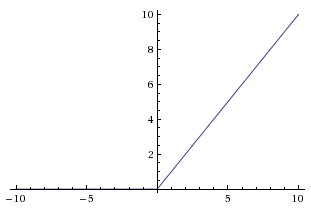
\includegraphics[width=0.5\textwidth]{figures/relu.jpeg}
				\caption{Función de activación \textit{\ac{ReLU}}.}
				\label{fig.reLu}
			\end{center}
		\end{figure} 
	\end{description}
	
\item[\textit{Loss Layers}] \hfill 
\vspace{10pt}
\\
	El cálculo de la pérdida permite el aprendizaje mediante la comparación de la salida con un objetivo y la asignación de un coste para minimizarla. Se calcula mediante el paso hacia adelante. Existen diferentes medidas de las que se destacan dos.
	\vspace{10pt}
	\begin{description}
	\item[\textit{Softmax with Loss}] \hfill 
	\vspace{5pt}
	\\
		La función \textit{softmax} se utiliza a menudo en la capa final de un clasificador basado en redes neuronales. Se trata de una función que modifica un vector K-dimensional de valores reales arbitrarios a un vector K-dimensional de valores reales en el rango (0, 1] que suman 1.\\
		\vspace{-10pt}
		\\
		Esta capa es conceptualmente idéntica a una capa de \textit{softmax}, la cual calcula la función con el mismo nombre, seguida por una capa de pérdida logística multinomial, proporcionando un gradiente numéricamente más estable.
		Se calcula l pérdida como: 
		$$E = \frac{-1}{N} \sum\limits_{n=1}^N \log(\hat{p}_{n,l_n})$$
		Siendo $N$ el número total de muestras, $\hat{p}$ las probabilidades de cada etiqueta para cada muestra y $l_n$ las etiquetas existentes. Se definen las etiquetas existentes como $l_n\in[0, 1, 2, ..., K-1]$, siendo $K$ el total de clases. Adicionalmente, se debe multiplicar todo por $-1$ ya que se aplica el logaritmo a una probabilidad, oscilante entre 0 y 1, obteniendo un resultado negativo, y el que se desea obtener debe ser positivo.
		\vspace{10pt}
	\item[Accuracy] \hfill 
	\vspace{5pt}
	\\
		Esta capa calcula únicamente la tasa de acierto de la red, es decir, el número de aciertos en la clasificación referenciado al número total de muestras analizadas.
		Se calcula como:
		$$\frac{1}{N} \sum\limits_{n=1}^N \delta\{ \hat{l}_n = l_n \}$$

		Donde $\hat{l_n}$ es la etiqueta que la red decide en la clasificación y, al igual que en el caso anterior, $N$  es el número total de muestras y $l_n$ las etiquetas existentes. Por último, la función $\delta\{x\}$ se define como:
		$$\delta\{ \textup{condición}\} = \left\{ \begin{array}{lr} 1 &  \textup{si condición} \\ 0 & \mbox{resto} \end{array} \right.$$
	\end{description}
	
\end{description}
\vspace{10pt}

Por último, además de las capas y parámetros definidos anteriormente, Caffe, permite el desarrollo de un solucionador (\textit{solver}) en el que se podrán ajustar parámetros como el número de iteraciones totales que se ejecutarán, el de evaluación que se van a realizar, cada cuantas iteraciones se realizará esa evaluación, o se sacarán redes intermedias.\\

Para Caffe, el número de iteraciones no se corresponde con el número de veces que la red recorre la base de datos al completo, sino como las veces que se pasa por cada lote al completo. Esto viene dado porque, debido a la amplia dimensión de las bases de datos necesarias para desarrollar el aprendzaje profundo, según se explicación en el Capítulo~\ref{cap.introduccion}, será necesaria una división de la misma en pequeños lotes para que ordenador no se bloquee en el tratamiento de las mismas. De esta manera, se define el número de épocas, es decir, el número de veces que se recorre de manera completa la base de datos, con la siguiente expresión:\\
$$\textup{N.Epocas}=\frac{\textup{Tamaño lote de entrenamiento}\times \textup{Total iteraciones}}{\textup{Muestras entrenamiento}} $$\\

\subsection{DroidCam}\label{sec.droid}
DroidCam~\footnote{https://www.dev47apps.com/} es una aplicación que permite convertir un dispositivo móvil en una cámara web, estableciendo una conexión mediante WiFi/LAN, modo servidor wifi, o USB. Esta aplicación es muy usada para establecer videoconferencias a través de plataformas como Skype o Google+, entre otras aplicaciones. En este trabajo será usada para obtener el flujo de vídeo desde un dispositivo distinto a la webcam del ordenador, haciendo más sencillo el manejo del mismo.\\

La aplicación funciona con un componente cliente en el ordenador que instala los controladores de la cámara web y conecta el equipo con el dispositivo Android, que deberá tener instalada la misma aplicación.\\

Entre sus características principales destacan:
	\begin{itemize}
		\item Incluye sonido e imagen
		\item Conexión por diferentes medios
		\item Uso de otras apliaciones con DroidCam en segundo plano
		\item Cámara IP de vigilancia con acceso MJPEG
	\end{itemize}

\vspace{10pt}
\section{Bases de datos}

\subsection{MNIST}\label{sec.minst}
La base de datos \textit{\ac{MNIST}}~\footnote{http://yann.lecun.com/exdb/mnist/} está formada por diferentes imágenes con números escritos a mano y consta de un conjunto de entrenamiento de 60.000 ejemplos y otro de prueba de 10.000 ejemplos. Es una buena base de datos para personas que quieren probar técnicas de aprendizaje y métodos de reconocimiento de patrones en datos del mundo real, mientras que dedican un mínimo esfuerzo a preprocesar y formatear. \\

Se trata de un subconjunto de una más grande, \textit{\ac{NIST}}, en la que las imágenes originales en blanco y negro fueron normalizadas en el tamaño para encajar en un cuadro de 20x20 píxeles, preservando su relación de aspecto. Las imágenes obtenidas contienen niveles de gris como resultado de la técnica anti-aliasing utilizada por el algoritmo de normalización. Estas imágenes se centraron en una de 28x28 calculando el centro de masa de los píxeles y trasladando la imagen para situar este punto en el centro del campo 28x28.\\

Fue construida a partir de la Base de Datos Especial 3 y la Base de Datos Especial 1 del \ac{NIST}, que contienen imágenes binarias de dígitos manuscritos. \ac{NIST} originalmente designó SD-3 como su conjunto de entrenamiento y SD-1 como su conjunto de pruebas. Sin embargo, SD-3 es mucho más limpio y más fácil de reconocer que SD-1.Esto es debido a que SD-3 fue recogido entre los empleados de la Oficina del Censo, mientras que el SD-1 fue recogido entre los estudiantes de secundaria. Dado que para una buena extracción de conclusiones es necesario que el resultado sea independiente de la elección del conjunto de entrenamiento y de prueba entre el conjunto completo de muestras, fue necesaria la elaboración de un nuevo conjunto en el que ambas bases de datos estuviesen representadas de manera equitativa. Además, se aseguraron de que los conjuntos de escritores en el de entrenamiento y el de prueba son disjuntos.\\

\subsection{COCO}
Microsoft \textit{\ac{COCO}}~\footnote{http://mscoco.org/} es un gran conjunto de datos de imágenes diseñado para la detección de objetos, segmentación y generación de subtítulos~\cite{veit2016cocotext}. Alguna de las características principales de este conjunto de datos son:
	\begin{itemize}
         \item Múltiples objetos en cada imagen
     	 \item Más de 300.000 imágenes
         \item Más de 2 millones de instancias
         \item 80 categorías de objetos
    \end{itemize}
    
Esta plataforma se ha desarrollado para varios retos, en concreto es de interés el reto de la detección, establecido en 2016. Se utilizan conjuntos de entrenamiento, prueba y validación con sus correspondientes anotaciones. \ac{COCO} tiene tres tipos de anotaciones: instancias de objeto, puntos clave de objeto y leyendas de imagen, que se almacenan utilizando el formato de archivo \textit{\ac{JSON}} y comparten estructura de datos establecida en la Figura~\ref{fig.basicStruc}. \\

\begin{figure}[H]
	\begin{center}
		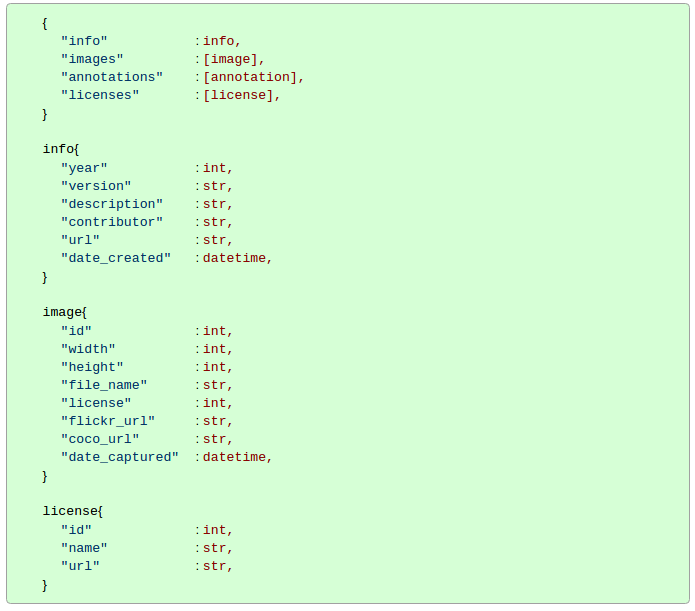
\includegraphics[width=0.8\textwidth]{figures/basic_structure_annotations.png}
		\caption{Estructura básica de anotaciones en \ac{COCO}.}
		\label{fig.basicStruc}
	\end{center}
\end{figure} 

Para la detección son de interés las anotaciones de instancias de objetos, cuya estructura se muestra en la Figura~\ref{fig.objInst}.Cada anotación de instancia contiene una serie de campos, incluyendo el ID de categoría y la máscara de segmentación del objeto. El formato de segmentación depende de si la instancia representa un único objeto (\textit{iscrowd}~=~0), en cuyo caso se utilizan polígonos, o una colección de objetos (\textit{iscrowd}~=~1), en cuyo caso se utiliza \textit{\ac{RLE}}. Debe tenerse en cuenta que un único objeto puede requerir múltiples polígonos, y que las anotaciones de la multitud se utilizan para etiquetar grandes grupos de objetos. Además, se proporciona una caja delimitadora para cada objeto, cuyas coordenadas se miden desde la esquina superior izquierda de la imagen y están indexadas en 0. Finalmente, el campo de categorías  almacena el mapeo del ID de categoría a los nombres de categoría y supercategoría.

\begin{figure}[H]
	\begin{center}
		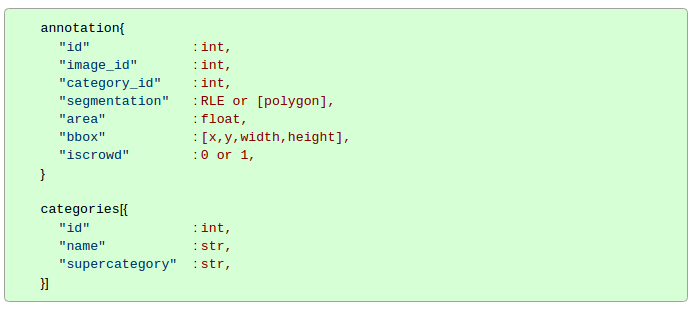
\includegraphics[width=0.8\textwidth]{figures/instancia_objetos.png}
		\caption{Estructura de instancias de objetos en \ac{COCO}.}
		\label{fig.objInst}
	\end{center}
\end{figure}

\subsection{VOC}
El objetivo del desafío de \textit{\ac{VOC}} \cite{Everingham10} es investigar el desempeño de los métodos de reconocimiento en un amplio espectro de imágenes naturales. Para ello, se requiere que los conjuntos de datos \ac{VOC} contengan variabilidad significativa en términos de tamaño del objeto, orientación, pose, iluminación, posición y oclusión. También es importante que los conjuntos de datos no muestren sesgos sistemáticos, por ejemplo, favoreciendo imágenes con objetos centrados o una buena iluminación. Del mismo modo, para garantizar un entrenamiento y una evaluación precisa, es necesario que las anotaciones de imagen sean consistentes, precisas y exhaustivas para las clases especificadas.\\

Teniendo claros estos conceptos, en 2007, se llevó a cabo una recolección de imágenes, como las mostradas en la Figura~\ref{fig.voc_example}, formando el conjunto de datos \textit{\ac{VOC}}\textit{2007}~\cite{pascal-voc-2007}. Este conjunto dispone de dos grandes bases de datos, una de ellas compuesta por un conjunto de validación y otro de entrenamiento, y la otra con un único conjunto de test. Ambas bases de datos contienen alrededor de 5000 imágenes en las que se representan, apróximadamente, 12.000 objetos diferentes, por lo que, en total, este conjunto dispone de unas 10000 imágenes en las que se reperesentan unos 24000 objetos. En el año 2012 se modifica este conjunto, aumentando a 11530 el número de imágenes con representación de 27450 objetos diferentes~\cite{pascal-voc-2012}.

\begin{figure}[H]
	\begin{center}
		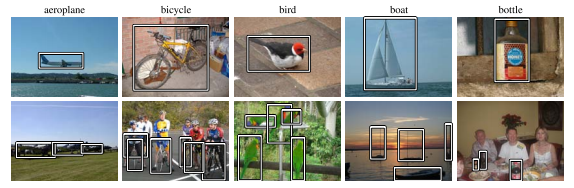
\includegraphics[width=0.7\textwidth]{figures/vocexample}
		\caption{Ejemplos de imágenes en \ac{VOC}. Imagen tomada de~\cite{Everingham10}}.
		\label{fig.voc_example}
	\end{center}
\end{figure}

Dado que la finalidad de este conjunto de datos es permitir el desarrollo tanto de la clasificación de objetos como la detección de los mismos, será necesario que estas imágenes contengan una serie de anotaciones. Entre otras cosas, estas anotaciones contienen dos atributos importantes para ambas tareas:

\begin{itemize}
	\item Para la \textbf{clasificación}, se debe indicar la clase de objeto que es. Los objetos de este conjunto estan clasificados en 20 clases diferentes. En la Figura~\ref{fig.clasesVOC} se puede observar la división que se hace de cada una de las clases y las distintas clases existentes.
	\item Para la \textbf{detección}, será necesario indicar, para cada objeto, la \textit{bounding box}. Se trata de un cuadro delimitador alineado con el eje que rodea la extensión del objeto visible en la imagen, permitiendo identificar el objeto en la imagen.
\end{itemize}
\begin{figure}[H]
	\begin{center}
		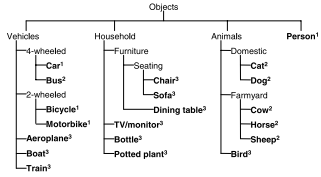
\includegraphics[width=0.7\textwidth]{figures/vocclasses}
		\caption{Estructura de las clases en \ac{VOC}2007. Imagen tomada de~\cite{Everingham10}}. El año de inclusión de cada clase en el desafío está indicado por
		superíndices: $2005^1$, $2006^2$, $2007^3$.
		\label{fig.clasesVOC}
	\end{center}
\end{figure}

\section{Evaluación de prestaciones} \label{sec.prestaciones}
Existen multitud de parámetros que permiten la evaluación de las redes neuronales, sin embargo, en este proyecto, todas las comparaciones se centrarán en cinco de ellas: \textit{accuracy}, \textit{loss}, matriz de confusión, \textit{precision} y \textit{recall}~\cite{pullum2007guidance}.\\

Las dos primeras fueron explicadas en la Sección~\ref{sec.caffe}, por lo que no se ahondará más sobre ellas. Las tres restantes serán explicdas más profundamente, y de manera totalmente teórica a continuación.

\subsection{Matriz de confusión}
Una matriz de confusión (Kohavi y Provost, 1998) contiene información sobre las clasificaciones reales y predichas hechas por un sistema de clasificación. El rendimiento de estos sistemas se evalúa comúnmente utilizando los datos de la matriz~\cite{metrics}. En la Figura~\ref{fig.matriz} se muestra un ejemplo sencillo de la construcción de esta matriz donde:
\begin{itemize}
	\item \textbf{\textit{a}} es el número de predicciones correctas de que una instancia es negativa
	\item \textbf{\textit{b}} es el número de predicciones incorrectas de que una instancia es positiva
	\item \textbf{\textit{c}} es el número de predicciones incorrectas de una instancia negativa
	\item \textbf{\textit{d}} es el número de predicciones correctas de que una instancia es positiva.
\end{itemize}

\begin{figure}[H]
	\begin{center}
		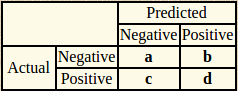
\includegraphics[width=0.3\textwidth]{figures/matrizexample}
		\caption{Ejemplo sencillo de matriz de confusión. Imagen tomada de~\cite{metrics}}.
		\label{fig.matriz}
	\end{center}
\end{figure}

Además de ayudar con el cálculo de \textit{precision} y \textit{recall}, es importante mirar la matriz de confusión para analizar sus resultados, ya que también proporciona información importante sobre dónde el clasificador funciona mal~\cite{metrics2}. Para que una matriz proporcione información sobre el correcto funcionamiento de un clasificador se obtendrán valores altos en la diagonal, y lo más pequeños posible en el resto de celdas de la misma.

\subsection{\textit{Precision}}
Se trata de la proporción de los casos positivos predichos que fueron correctos~\cite{metrics}. Para obtener este valor en el ejemplo sencillo anteriormente explicado se utiliza la fórmula:
$$P = \frac{d}{b+d} $$
Donde $P$ es el valor de \textit{precision} y $b$ y $d$ los mismo valores explicados en la sección anterior.\\

En un caso más complejo en el que la clasificación no sea binaria, se deben de tener en cuenta todas las clases, por ello la fórmula queda expresada de la siguiente forma~\cite{metrics2}:
$$P = \frac{TP_X}{TP_X + FP_X} $$
Donde:
\begin{itemize}
	\item $TP_X$ se corresponde el número de verdaderos positivos para la clase $X$, es decir, el valor de aciertos correspondiente para dicha clase, situado en la diagonal.
	\item $FP_X$ se corresponde el número de falsos positivos para la clase $X$, es decir, el número de veces que se predijo dicha clase sin haber sido producida, correspondiente con la suma del resto de celdas en la misma fila.
\end{itemize}

\subsection{\textit{Recall}}
Se trata de la proporción de casos positivos que fueron correctamente identificados~\cite{metrics}. Para el ejemplo sencillo se calcula mediante la siguiente expresión:
$$R = \frac{d}{c+d} $$
Donde $R$ es el valor de \textit{recall} y $c$ y $d$ los mismo valores explicados anteriormente.\\

Al igual que en el caso de la sección anterior, en caso de tener una clasificación multiclase se deberás tener en cuenta todas ellas, utilizando para ello la expresión~\cite{metrics2}:
$$R = \frac{TP_X}{TP_X +FN_X} $$
Donde $TP_X$ se corresponde con lo explicado en la sección anterior y $FN_X$ se corresponde con los falsos negativos para la clase $X$, es decir, el número de veces que se predijo errónamente otra clase habiéndose producido $X$, correspondiente con la suma del resto de la columna. 
\lhead[]{CAPÍTULO \thechapter. CLASIFICACIÓN}
\chapter{Clasificación con Aprendizaje Profundo}\label{cap.clasificacion}
En este capítulo se expondrá el trabajo realizado para la comprensión del problema de clasificación de imágenes utilizando una plataforma de aprendizaje profundo. Para ello se ha elaborado un componente en Python que permite la clasificación de dígitos del 0 al 9 en tiempo real, que ha sido mejorado gracias a un amplio estudio sobre las variantes posibles aplicadas a las redes entrenadas, utilizando la plataforma Caffe.\\

\section{Clasificador de dígitos}
La primera tarea que se abarca en el proyecto es el desarrollo de un componente en Pyhton para la clasificación de dígitos entre 0 y 9 en tiempo real, materializando en una aplicación concreta el probblema de la clasificación de imágenes con aprendizaje profundo. Para poder desarrollar esta aplicación es necesario, previamente, un entendimiento de una primera red básica, que será la encargada de realizar la clasificación. En esta sección se explicará el procedimiento seguido para el entendimiento de la red y el desarrollo del propio componente.\\

\subsection{Red básica}\label{sec.red}
La red que se empleará, está orientada a la clasificación de números utilizando, en el entrenamiento, la base de datos numérica MNIST, explicada en la Sección~\ref{sec.minst}, y en la que se entrará en detalle a continuación.\\

La base de datos explicada, MNIST, proporciona dos conjuntos de datos, uno de entrenamiento y otro de test, pero, a diferencia de otros conjuntos no dispone de una de validación, utilizada para evaluar el modelo durante el entrenamiento. Por ello, el primer paso que se derá consiste en dividir la base de datos de entrenamiento en dos, obteniendo un conjunto de validación a partir del que ofrece MNIST para el entrenamiento. Para esta tarea, se desarrolla un script, \textit{createvalidationdatabase.py}, que divide la base de datos de entrenamiento original en dos, el 80\% para entrenamiento y el 20\% restante para validación. En la Tabla~\ref{tab.baseDatos}, se muestra un resumen de la estructura final de ambas bases de datos, así como la estructura de la base de datos de test que no sufre ninguna modificación.\\

\begin{table}[H]
	\centering
	\begin{tabular}{|l|c|c|c|c|}
		\hline
		\textbf{Dígito} & \textbf{Total} & \textbf{80\%} & \textbf{20\%} & \textbf{Test}\\
		\hline \hline
		0 & 5923 & 4738 & 1185 & 980\\ \hline
		1 & 6742 & 5393 & 1349 & 1135\\ \hline
		2 & 5958 & 4767 & 1191 & 1032\\ \hline
		3 & 6131 & 4905 & 1226 & 1010\\ \hline
		4 & 5842 & 4674 & 1168 & 982\\ \hline
		5 & 5421 & 4337 & 1084 & 892\\ \hline
		6 & 5918 & 4734 & 1184 & 958\\ \hline
		7 & 6265 & 5012 & 1253 & 1028\\ \hline
		8 & 5851 & 4681 & 1170 & 974\\ \hline
		9 & 5949 & 4759 & 1190 & 1009\\ \hline
		Total & 60000 & 48000 & 12000 & 10000\\ \hline
	\end{tabular}
	\caption{Estructura de conjuntos de datos.}
	\label{tab.baseDatos}
\end{table}

Se puede comprobar, como era de esperar, que no todos los dígitos tienen la misma presencia, siendo mayor el número de muestras en los dígitos que pueden generar mayor confusión, como el 1 o el 7, y menor en los que son más claros como el 0. Por ello, es muy importante respetar las proporciones existentes en cada dígito el dividir la base de datos para no alterar la naturaleza de la base de datos original. Para mantener esta proporción se calculará el porcentaje sobre el total de cada dígito y no sobre el total del conjunto de datos.\\

En la Figura~\ref{fig.digitosMNIST} se puede observar una muestra de cada uno de los dígitos que se almacenan, en este caso, en la base de datos de test, siendo de las mismas características el resto de bases de datos explicadas.

\begin{figure}[H]
	\begin{center}
		
\includegraphics[width=0.3\textwidth]{figures/original}
		\caption{Muestras de base de datos MNIST original.}
		\label{fig.digitosMNIST}
	\end{center}
\end{figure}

Tras tener claro los diferentes conjuntos de datos que se emplearán en adelante, se procede al entrenamiento de la red. Para entrenar una red, Caffe proporciona tres archivos que se editarán para adaptar la red al problema que se abarque. A continuación, se explicará cada uno de esos archivos, siguiendo el orden que fue necesario hasta conseguir la red completamente entrenada.\\

\subsubsection{Definición de la red}
	Caffe utiliza el archivo 
	\textit{lenet\_train\_test.prototxt} para la especificación de todos los parámetros que son necesarios en el entrenamiento de la red, es decir, en este documento se definen las imágenes que se emplearán, la propia estructura de la red y la forma en la que se analizarán las imágenes proporcionadas, todo ello empleando diferentes capas (\textit{layers}).\\

	La primera línea de este documento es utilizada para indicar el nombre que se le quiere dar a la red, según se muestra a continuación.
	\vspace{10pt}
	\begin{lstlisting}[frame=single]
	name: "LeNet"
	\end{lstlisting}
	
	En concreto, esta red recibe el nombre de LeNet, un tipo de red que es conocida por un buen funcionamiento en las tareas de clasificación de dígitos y que, por lo general, consta de una capa convolucional seguida por una capa de agrupamiento (\textit{pooling}), repetido dos veces. Tras ellas, se incluyen dos capas totalmente conectadas similares a las perceptrones multicapa convencionales. Con Caffe la estructura habitual de la red LeNet se ve ligeramente modificada, pues se utiliza una función de activacion lineal en lugar de sigmoidal.\\

	Tras la definición del nombre se definen dos capas de datos, una de ellas correspondiente a los datos de entrenamiento y, la otra, correspondiente a los datos que se utilizarán para realizar la evaluación durante el entrenamiento, obteniendo datos de \textit{accuracy} y \textit{loss} con el conjunto de validación. A continuación se muestra un ejemplo de cómo se define esta capa de datos, en concreto, en fase de entrenamiento.
	\vspace{10pt}
	\begin{lstlisting}[frame=single]
	layer {
		name: "mnist"
		type: "Data"
		top: "data"
		top: "label"
		include {phase: TRAIN}
		transform_param {scale: 0.00390625}
		data_param {
			source: "examples/mnist/mnist_train_lmdb"
			batch_size: 64
			backend: LMDB }
	}
	\end{lstlisting}
	
	Los parámetros de transformación (\textit{transform\_param}), indican el preprocesamiento de la imagen antes de comenzar el entrenamiento, y, éstos, deben coincidir en ambas fases, ya que si se evaluase la red con una transformación de la imágen distinta a la aplicada en el entrenamiento los resultados obtenidos no serían reales. En este caso, se utiliza un factor de escala, indicado con el nombre \textit{scale}, que establece el rango de la imagen en [0,1]. \\
	En esta red se utilizarán dos capas de datos que difieren en la fase en la que se utilizan los datos, entrenamiento o evaluación de la red, el tamaño del lote, siendo 64 muestras para el entrenamiento y 100 para la evaluación, y la ruta de la que se cogen los datos.\\
	
	A continuación, se comienzan a definir las capas del entrenamiento propiamente dicho. Se intercala una capa de convolución con una de agrupamiento y se repite la estructura dos veces.\\
	
	En la capa de convolución, explicada en la Sección~\ref{sec.caffe}, se define que el tamaño del filtro será de 5x5 y que se obtendrán 20 salidas en la primera de ellas, en la segunda, sin embargo, se obtendrán 50 salidas. Además se define el algoritmo "Xavier" para la inicialización de los pesos, que determina automáticamente la escala de inicialización basada en el número de entradas y de las neuronas de salida, y la inicialización del \textit{bias} mediante una constante que por defecto es 0. Esta estructura se define de la siguiente forma en el documento de Caffe:
	\vspace{10pt}
	\begin{lstlisting}[frame=single]
	layer {
		name: "conv1"
		type: "Convolution"
		bottom: "data"
		top: "conv1"
		param {lr_mult: 1}
		param {lr_mult: 2}
		convolution_param {
			num_output: 20
			kernel_size: 5
			stride: 1
			weight_filler {type: "xavier"}
			bias_filler {type: "constant"}
		}
	}	
	\end{lstlisting}
	
	La capa de agrupamiento, también explicada en la Sección~\ref{sec.caffe}, será alimentada por la capa de convolución anterior y alimentará a la siguiente en caso de que la haya. En caso de ser la última de las capas de agrupamiento sus salidas serán la entrada de las capas completamente conectadas cuya estructura se explicará más adelante en esta sección y que fueron detalladas en la Sección~\ref{sec.caffe}. Se definen en ella un tamaño de filtro de 2x2, un intervalo de dos muestras entre cada aplicación del filtro, por lo que no hay solape, y el método del máximo para realizar el agrupamiento. A continuación se muestra un ejemplo de cómo se define esta capa en el documento que se está tratando.
	\vspace{10pt}
	\begin{lstlisting}[frame=single]
	layer {
		name: "pool1"
		type: "Pooling"
		bottom: "conv1"
		top: "pool1"
		pooling_param {
			pool: MAX
			kernel_size: 2
			stride: 2 }
	}	
	\end{lstlisting}

	Como se mencionó anteriormente, tras estas capas se establecen las dos capas completamente conectadas, \textit{InnerProduct} cuya definición en el documento queda de la siguiente manera: 
	\vspace{10pt}
	\begin{lstlisting}[frame=single]
	layer {
		name: "ip1"
		type: "InnerProduct"
		bottom: "pool2"
		top: "ip1"
		param {lr_mult: 1}
		param {lr_mult: 2}
		inner_product_param {
			num_output: 500
			weight_filler {type: "xavier"}
			bias_filler {type: "constant"}
		}
	}	
	\end{lstlisting}
	
	En estas capas se definen 500 salidas para la primera de ellas, y tantas como clases se tengan, en la segunda. La aplicación que se está desarrollando pretende clasificar los dígitos del 0 al 9, por lo que esta última capa deberá de tener 10 salidas.\\

	Las capas completamente conectadas están separadas entre sí por una capa de activación, en este caso linear, llamada \textit{ReLu}. Esta capa fue explicada en la Sección~\ref{sec.caffe} y tiene la siguiente forma en el documento:
	\vspace{10pt}
	\begin{lstlisting}[frame=single]
	layer {
		name: "relu1"
		type: "ReLU"
		bottom: "ip1"
		top: "ip1"
	}	
	\end{lstlisting}
	
	Esta capa no dispone de ningún parámetro modificable ya que la plataforma proporciona directamente la función por su identificador único.\\
	
	Para terminar la estructura de la red básica, Caffe permite la opción de añadir capas que muestren parámetros de evaluación de la red que se está entrenando. Estas capas, se deben añadir como una capa más a continuación de las anteriormente explicadas y se definirá su estructura de la siguiente forma:
	\vspace{10pt}
	\begin{lstlisting}[frame=single]
	layer {
		name: "accuracy"
		type: "Accuracy"
		bottom: "ip2"
		bottom: "label"
		top: "accuracy"
		include {phase: TEST}
	}
	
	layer {
		name: "loss"
		type: "SoftmaxWithLoss"
		bottom: "ip2"
		bottom: "label"
		top: "loss"
	}	
	\end{lstlisting}
	
	Estas dos capas permiten obtener valores de precisión y pérdidas cada ciertas iteraciones, siendo marcado este valor en el documento que se explicará a continuación, el solucionador.\\

	En la Figura~\ref{fig.redBasica} se puede observar un esquema de la estructura definida en este apartado, los valores de interés y cada una de las entradas y salidas de las capas. Para obtener esta figura, se ha ejecutado un código proporcionado por la propia plataforma, que, mediante el archivo que define la estructura, explicado anteriormente, dibuja la red. Para ello se debe ejecutar el siguiente comando:
	\vspace{10pt}
	\begin{lstlisting}[frame=single]
	$ caffe/python/draw_net.py <netprototxt_filename> <out_img_filename>
	\end{lstlisting}
	
	\begin{figure}[H]
		\begin{center}
			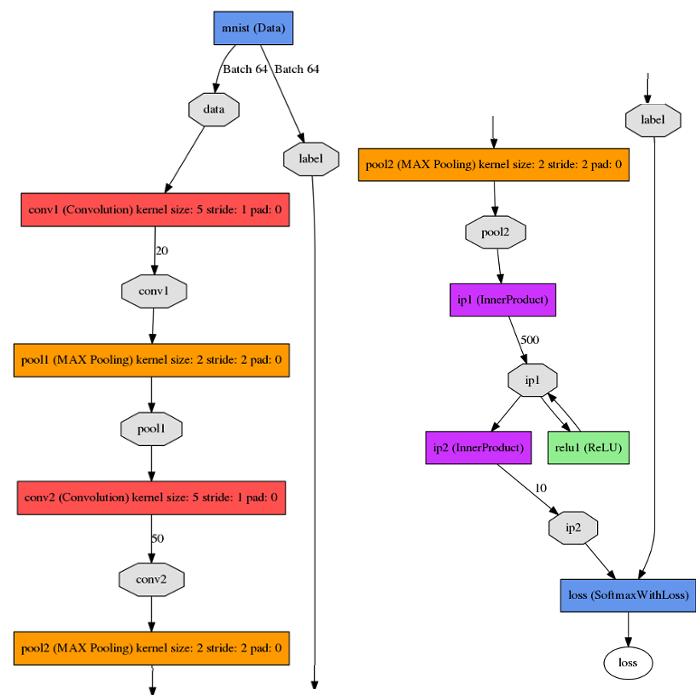
\includegraphics[width=0.8\textwidth]{figures/Original_net}
			\caption{Red básica LeNet MNIST.}
			\label{fig.redBasica}
		\end{center}
	\end{figure}
	
\subsubsection{Definición del solucionador}
	Para esta tarea se va a utilizar el archivo de Caffe \textit{lenet\_solver.prototxt}. En este documento se definen parámetros como la estructura de red que se utilizará, definida en el apartado anterior, y el número de iteraciones que se ejecutarán durante el entrenamiento de la red, cuya explicación se aportó en la Sección~\ref{sec.caffe}. Además, en ese mismo capítulo, se explican el resto de parámetros que se manejarán en este proyecto, como la evaluación de la red o las redes intermedias que se guardarán.
	\vspace{10pt}
	\begin{lstlisting}[frame=single]
	# The train/test net protocol buffer definition
	net: "examples/mnist/lenet_train_test.prototxt"
	# test_iter specifies how many forward passes the test should carry 
	# out.
	# In the case of MNIST, we have test batch size 100 and 100 test
	# iterations, covering the full 10,000 testing images.
	test_iter: 100
	# Carry out testing every 500 training iterations.
	test_interval: 500
	# The base learning rate, momentum and the weight decay of the network.
	base_lr: 0.01
	momentum: 0.9
	weight_decay: 0.0005
	# The learning rate policy
	lr_policy: "inv"
	gamma: 0.0001
	power: 0.75
	# Display every 100 iterations
	display: 100
	# The maximum number of iterations
	max_iter: 10000
	# snapshot intermediate results
	snapshot: 5000
	snapshot_prefix: "examples/mnist/lenet"
	# solver mode: CPU or GPU
	solver_mode: CPU	
	\end{lstlisting}
	
	Se debe fijar especial atención en parámetros como \textit{net}, que define la ruta al documento de la sección anterior en el que se define la estructura de red, \textit{test\_interval}, que marca cada cuántas iteraciones se realizará la evaluación de la red en el entrenamiento, \textit{max\_iter}, que define el número de iteraciones totales para finalizar el entrenamiento, \textit{snapshot}, que indica cada cúantas iteraciones se creará un archivo con la red intermedia correspondiente, y, finalmente, \textit{snapshot\_prefix}, que marcará la ruta en la que se almacenarán los archivos. La forma en la que se almacenan los archivos se corresponden con la ruta indicada hasta el último "\text{/}", siendo lo posterior el nombre deseado que será completado con el número de iteración correspondiente. En el ejemplo mostrado, el archivo será almacenado en la ruta \textit{"\text{examples/mnist/}"}    y el nombre de la red final será \textit{"lenet\_iter\_10000"}.\\
	
	Tras definir el solucionador se procederá a la ejecución de un archivo que comience con el entrenamiento de la red y permita obtener, finalmente, el modelo entrenado para usar en la aplicación.\\
	
\subsubsection{Ejecución de la red}
	Para comenzar con el entrenamiento de la red, una vez definida la estructura y y el solucionador, se deben ejecutar los siguientes comandos:
	\vspace{10pt}
	\begin{lstlisting}[frame=single]
	cd $CAFFE_ROOT
	./examples/mnist/train_lenet.sh	
	\end{lstlisting}
	
	El archivo que se ejecuta contiene información sobre qué solucionador se debe implementar y el modo de ejecución, de la forma que se muestra a continuación.
	\vspace{10pt}
	\begin{lstlisting}[frame=single]
	#!/usr/bin/env sh
	set -e
	
	./build/tools/caffe train 
	  --solver=examples/mnist/lenet_solver_validation.prototxt 
	\end{lstlisting}
	Este archivo, permite añadir una nueva línea mediante la que se obtiene, en la ruta marcada, un archivo de \textit{log} con información sobre el entrenamiento y la evaluación. Esta línea se añade tras indicar el solucionador de la forma que se muestra a continuación.
	\vspace{10pt}
	\begin{lstlisting}
		2>&1 | tee /home/nuria/TFG/logs/RedBasica.log $@
	\end{lstlisting} 
	
	En la Figura~\ref{fig.entrenamiento} se muestra la información que se observa en el terminal al ejecutar el entrenamiento, siendo ésta la misma que queda registrada en el archivo \textit{log} indicado.
	
	\begin{figure}[H]
		\begin{center}
			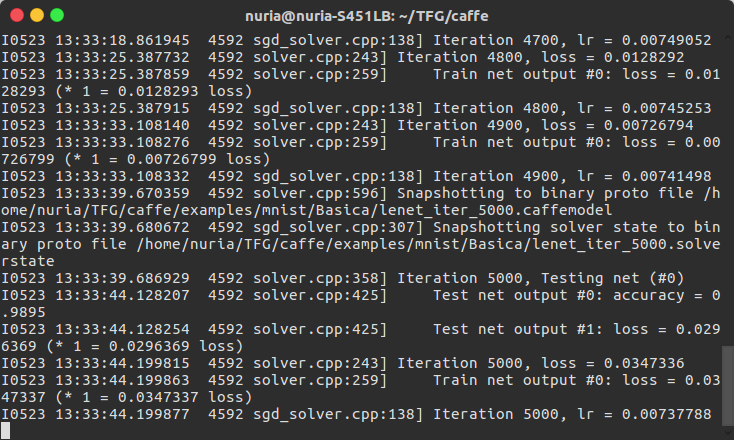
\includegraphics[width=0.8\textwidth]{figures/RedBasica5000}
			\caption{Ejecución de entrenamiento de red LeNet MNIST.}
			\label{fig.entrenamiento}
		\end{center}
	\end{figure}
	
	\begin{figure}[H]
		\begin{center}
			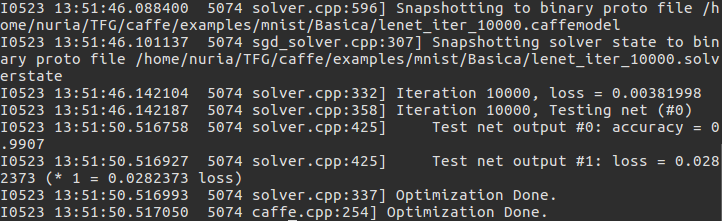
\includegraphics[width=0.8\textwidth]{figures/RedBasicaFin}
			\caption{Fin de entrenamiento de red LeNet MNIST.}
			\label{fig.finEntrBas}
		\end{center}
	\end{figure}
	
	Tras terminar el entrenamiento, mostrado en la Figura~\ref{fig.finEntrBas}, se obtiene el archivo con la red neuronal entrenada, almacenado según la ruta que se indicó en el solucionador, que podrá ser utilizada en la herramienta que sea de interés.\\

	Los parámetros de pérdidas y precisión calculados durante el entrenamiento para ambas fases, queda almacenados en el archivo \textit{log} generado, y serán divididos en las dos fases, entrenamiento y evauación para su análisis. Para ello se ejecuta el archivo \textit{parse\_log.sh} proporcionado por la plataforma en su carpeta \textit{tools/extra}. En la Figura~\ref{fig.parse} se muestra el aspecto de estos archivos desglosados.
	\vspace{10pt}
	
	\begin{figure}[H]
			\centering
			\subfigure[Entrenamiento]{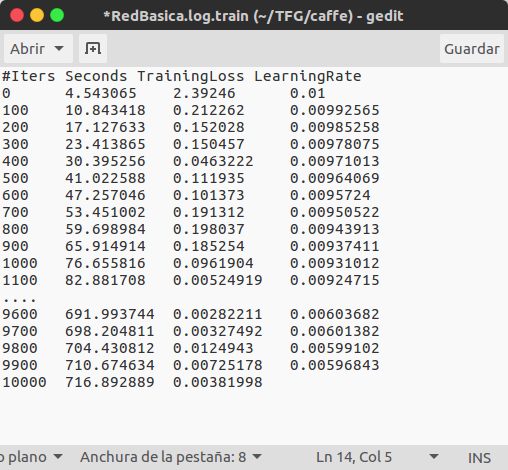
\includegraphics[width=0.4\textwidth]{figures/parselogtrain}} \hspace{10pt}
			\subfigure[Evaluación]{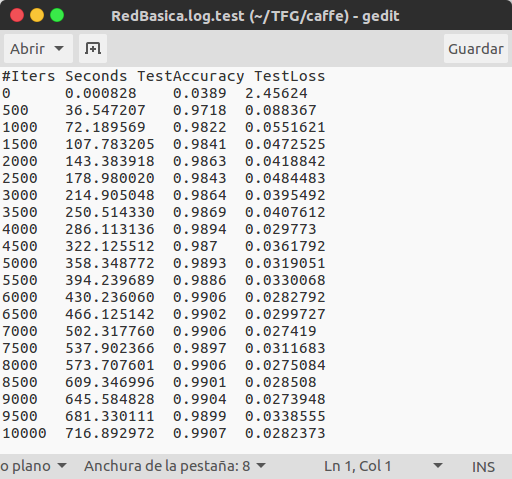
\includegraphics[width=0.4\textwidth]{figures/parselogtest}}
			\caption{Archivos \text{log}.}
			\label{fig.parse}
	\end{figure}

\subsection{Componente Python} \label{sec.componente}
Se ha desarrollado un componente escrito en Python que, mediante la ayuda del \textit{Camera Server} de JdeRobot, comentado en la Sección~\ref{sec.jderobot},  y la red explicada en la Sección~\ref{sec.red}, es capaz de clasificar un dígito mostrado a la cámara, que se especificará en un archivo de configuración, en tiempo real, encendiendo una bombilla que se corresponde con el número obtenido.\\

Debido a la magnitud de la tarea a realizar, se optó por dividir el programa en dos hilos que serán explicados a continuación. Uno de ellos se encargará del aspecto gráfico de la aplicación, mostrando la imagen obtenida por la cámara, la imagen procesada para la clasificación, y la iluminación de la bombilla correspondiente. El segundo hilo, se encargará de gestionar la captación de la cámara, mediante la conexión con el componente \textit{Camera Server}, así como el proceso de clasificación, utilizando la red entrenada. Todo el código correspondiente a esta aplicación podrá ser encontrado en~\cite{codigo}.\\

\subsubsection{Cámara} \label{sec.camara}
El hilo fundamental de la aplicación, que se encargará de la lógica de la misma mediante la adquisición de la imagen y su posterior procesamiento, estará referenciado por el nombre \textit{Camera}.\\

Al comienzo de la ejecución se inicializa un objeto Cámara, mediante el constructor \textit{Camera()}, que será el encargado de gestionar las acciones anteriormente nombradas. En esta inicialización se indica qué cámara se va a utilizar, referenciada de manera externa mediante un archivo de configuración que se indicará en la ejecución de la aplicación. La línea que indica la cámara en este archivo es la siguiente:
\vspace{10pt}
\begin{lstlisting}[frame=single]
	Numberclassifier.Camera.Proxy=cameraA:default -h localhost -p 9999
\end{lstlisting}

Esta propiedad estará enlazada con el componente \textit{Camera Server} de JdeRobot que nos proporciona un servidor de imágenes mediante la cámara.\\

Otro aspecto importante que se maneja en la inicialización de la cámara es la especificación y carga de la red que se empleará para la clasificación. Este aspecto se realiza mediante las siguientes líneas:
\vspace{10pt}
\begin{lstlisting}[frame=single]
	model_file = '/home/nuria/TFG/caffe/examples/mnist/lenet.prototxt'
	pretrained_file = '/home/nuria/TFG/caffe/examples/mnist/Basica/
						/lenet_iter_10000.solverstate'
	self.net = caffe.Classifier(model_file, pretrained_file, 
									image_dims=(28, 28), raw_scale=255)
\end{lstlisting}

Con este código se realizan las tres acciones necesarias para establecer la red que se utilizará. En primer lugar, se indica cuál será el modelo empleado para la clasificación. Este modelo es un archivo porporcionado por Caffe de manera homóloga al \textit{lenet\_train\_test.prototxt}, con la excepción de que la capa de datos no recurre a archivos almacenados sino que utiliza imágenes que serán insertadas en la ejecución de la red. El resto de datos deben ser exáctamente iguales a la estructura de la red entrenada para que no se produzcan errores. En segundo lugar, se indica la red entrenada que se utilizará en la ejecución, el archivo obtenido al finalizar el entrenamiento según se indicó en la Sección~\ref{sec.red}. Por último, se crea la red ejecutable, es decir, se crea un objeto que será utilizado por la aplicación cada vez que se quiera realizar la clasificación. Para esta creación es necesario indicar, en primer lugar, que se trata de una red para la clasificación, y, además, introducir los parámetros del modelo, la red entrenada, las dimensiones de las imágenes, y la escala de los píxeles.\\

Además de las propiedades más importantes comentadas anteriormente, se definen también funciones que serán importantes para la ejecución de la aplicación. Se establece una función \textit{update(self)}, que será llamada cada 150ms para la actualización del hilo \textit{ThreadCamera(camera)}, creado en el componente principal, para obtener las imágenes de forma periódica y poder establecer un flujo de vídeo a tiempo real. Esta función, a su vez, necesita de otra, \textit{getImage(self)}, que obtiene la imagen, la redimensiona, y le aplica una transformación necesaria antes de introducirla en el proceso de clasificación, devolviendo un array con las dos imágenes, original y transformada. Para esa transformación se utiliza una tercera función de la cámara, \textit{trasformImage(self,img)}. En ella, se centra la imagen en un cuadrado, pues la captada es rectangular y la necesaria para introducir en la red debe ser cuadrada, se convierte a imagen de grises, se redimensiona al tamaño necesario para introducirla en la red (28x28), y por último, se le aplica un filtro gaussiano de 5x5 para reducir el ruido.\\

Finalmente, se crea la siguiete función para realizar la clasificación de los dígitos:
\vspace{10pt}
\begin{lstlisting}[frame=single]
	def classification(self, img):
		self.net.blobs['data'].reshape(1,1,28,28)
		self.net.blobs['data'].data[...]=img * 0.00390625
		output = self.net.forward()
		digito = output['prob'].argmax()
		return digito
\end{lstlisting}

En primer lugar se asegura que las dimensiones del \textit{bolb} de datos sea de 28x28. En el siguiente paso, se introduce a la red la imagen obtenida tras la transformación, aplicandole el factor de escala para que el intervalo de los píxeles esté entre 0 y 1, pues eso fue lo que se indicó en el aprendizaje. Posteriormente se ejecuta la red y se obtiene, como salida, una estructura que almacena, por un lado, la propiedad \textit{'prob'} que se corresponde con un array que incluye las probabilidades de que la imagen introducida sea cada uno de los dígitos posibles, y, por otro, el tipo de datos que se almacena, en este caso \textit{float32}. Posteriormente, de ese array de probabilidades, se escoge el dígito cuya probabilidad es mayor, es decir, la clasificación realizada, y se devuelve.\\

Una vez establecida la lógica de la aplicación, con las funciones explicadas anteriormente, se procede a desarrollar el interfaz gráfico que permite al usuario visualizar, tanto las imágenes captadas y transformadas, como el resultado de la clasificación.\\

\subsubsection{GUI}
Para el aspecto gráfico de la aplicación, en el componente principal, se inicializará un objeto llamado \textit{window} mediante el constructor \textit{Gui()}, al que posteriormente se le vinculará la cámara mediante una función propia, \textit{window.setCamera(camera)}. Por último, al tratarse de un componente gráfico, será necesario indicar que se muestre mediante \textit{window.show()}. Al inicializar este objeto se crean todos los elementos gráficos que serán necesarios y que se modificarán posteriormente para conseguir el resultado deseado.\\

Al igual que en el caso de la cámara, se estabelcerá un hilo que permita aligerar la ejecución de la aplicación mediante \textit{ThreadGui(window)}, que establece el tiempo de actualización en 50ms. Debido al uso de este hilo, se crea en el objeto una función \textit{update()} que, en este caso, se encarga de obtener las imágenes original y transformada mediante la función \textit{getImage()} de la cámara, y adaptarlas para poder mostrarlas en las etiquetas definidas para cada una de ellas. Además, llama a otra función propia, \textit{lightON(out)}, que cambia el color del fondo del dígito que se haya clasificado, haciendo uso de la función de clasificación definida anteriormente en la cámara.\\

En la Figura~\ref{fig.gui} se puede observar el resultado gráfico de la aplicación. Al no tener detección, la ejecución de la clasificación es continua, por lo que, aunque no exista un dígito en la imagen, el componente decide constantemente un determinado dígito que considerará correcto, encendiendo la bombilla adecuada.\\

\begin{figure}[H]
	\begin{center}
		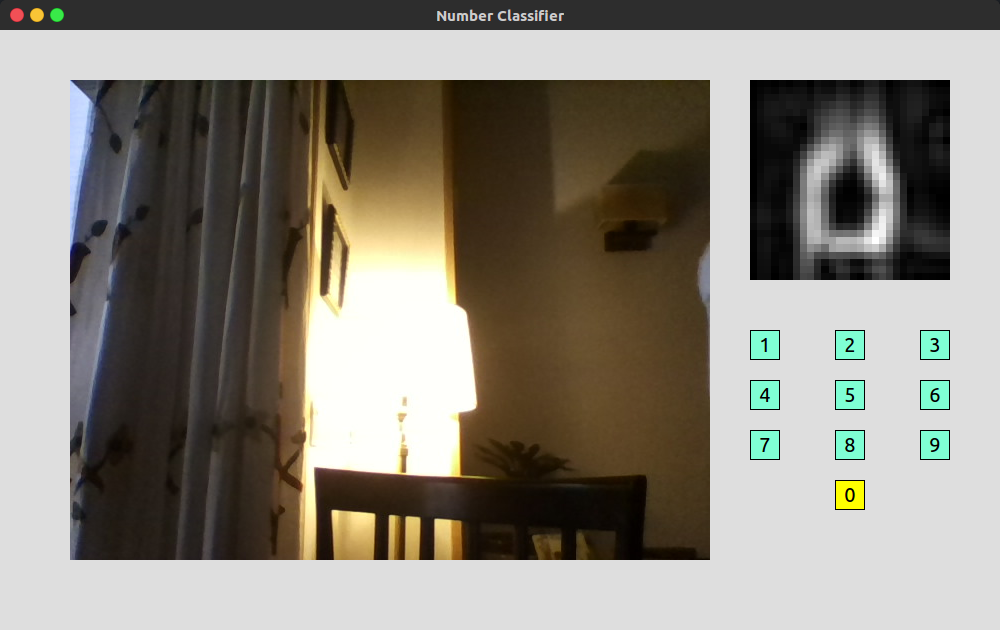
\includegraphics[width=0.8\textwidth]{figures/gui}
		\caption{Captura de componente gráfico de la aplicación.}
		\label{fig.gui}
	\end{center}
\end{figure}

\subsubsection{Ejecución}
El proceso de ejecución del componente se divide en dos pasos. Por un lado, será necesaria la ejecución del servidor de imágenes, para lo que se utilizará el componente de JdeRobot. Por otro lado se debe lanzar el propio componente clasificador explicado anteriormente.\\

Para ejecutar el \textit{Camera Server}, se seguirán las instrucciones que aporta la plataforma JdeRobot, utilizando el archivo de configuración que se facilita. Se utilizará el siguiente comando: 
\vspace{10pt}
\begin{lstlisting}[frame=single]
	cameraserver cameraserver.cfg
\end{lstlisting}

En el desarrollo de este trabajo, la propiedad de interés del archivo de configuración es \textit{CameraSrv.Camera.0.Uri}, que se centra en indicar la fuente de vídeo. Esta fuente puede ser un archivo de vídeo almacenado, para el que se empleará la ruta del archivo en ese campo, la webcam del propio ordenador, para el que se utilizará el valor 0, u otra cámara externa, para la que se le indicará el valor 1.\\

En la Sección~\ref{sec.droid} se comentó una aplicación que permitía utilizar la camara de un smartphone android como fuente de vídeo mediante una cámara externa. Para poder utilizar esta herramienta es necesario tener instalados el programa tanto en el dispositivo móvil a utilizar como en el propio ordenador, según se indica en la guía de la aplicación~\footnote{https://www.dev47apps.com/droidcam/linuxx/}, y abrir la aplicación. Una vez abierta en ambos dispositivos, se debe conectar el USB del ordenador al móvil e indicar en la aplicación de escritorio que la conexión se hará vía USB. La razón del uso del USB y no de la conexión vía \textit{WiFi} radica en la rapidez, siendo más adecuada para tiempo real. Una vez se han realizado las acciones anteriores se estable la conexión y se obtienen los resultados de la Figura~\ref{fig.droid} para el ordenador y el dispositivo.

\begin{figure}[H]
	\centering
	\subfigure[Escritorio]{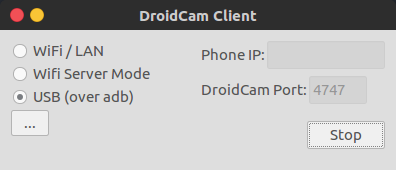
\includegraphics[width=0.4\textwidth]{figures/droidcamEscr}} \hspace{10pt}
	\subfigure[Dispositivo móvil]{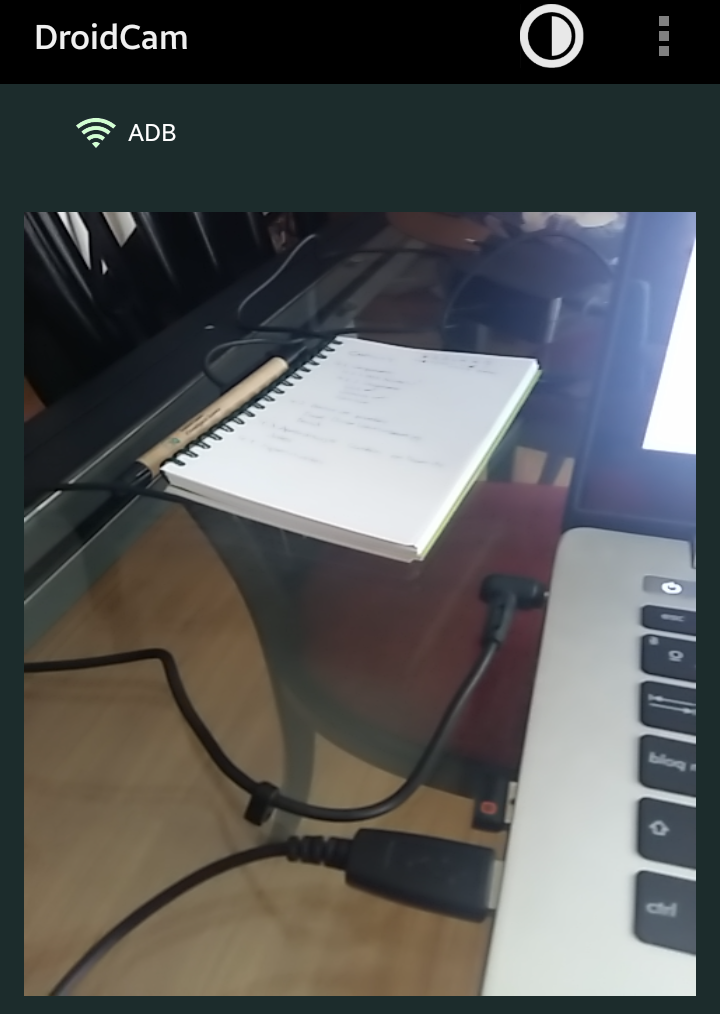
\includegraphics[width=0.3\textwidth]{figures/droidcamMov}}
	\caption{Capturas de DroidCam en los diferentes dispositivos}
	\label{fig.droid}
\end{figure}

Tras tener en funcionamiento el servidor de imágenes se debe proceder a la ejecución del componente clasificador, para ello se ejecutará el siguiente comando:
\vspace{10pt}
\begin{lstlisting}[frame=single]
	python numberclassifier.py --Ice.Config=numberclassifier.cfg
\end{lstlisting}

El componente Python contiene los procedimientos indicados en las secciones anteriores, la creación del GUI, la cámara y el lanzamiento de los hilos correspondiente a cada uno de ellos. En el fichero de configuración se tiene una porpiedad que indica qué cámara utilizar, es importante que el nombre de esta cámara se corresponda con el indicado en el fichero de configuración del servidor, de esta manera se establece la comunicación entre ambos componentes.\\

Finalmente, tras la ejecución, obtenemos el resultado del componente mostrado en la Figura~\ref{fig.componente1}, donde se aprecia el funcionamiento del mismo para un número sencillo y perfectamente definido según el entrenamiento de la red, es decir, fondo negro y número blanco.

\begin{figure}[H]
	\begin{center}
		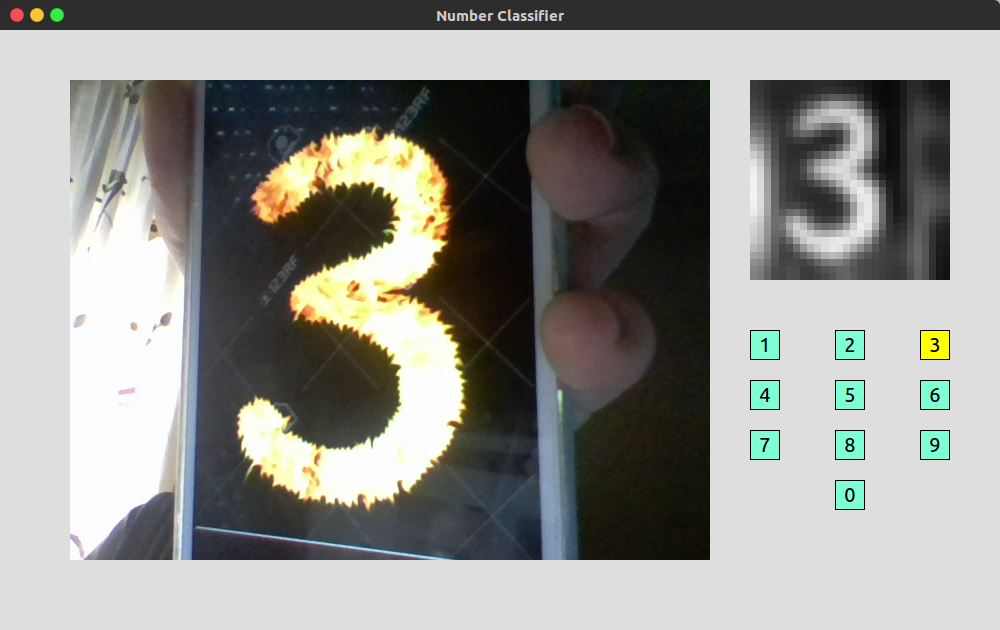
\includegraphics[width=0.5\textwidth]{figures/componente1}
		\caption{Captura del componente clasificador.}
		\label{fig.componente1}
	\end{center}
\end{figure}

Tras conseguir la aplicación del clasificador, se ha evaluado la red obtenida mediante un banco de pruebas, que será explicado a continuación y se ha procedido a la mejora de la misma gracias a los diferentes resultados obtenidos.\\

\section{Banco de pruebas} \label{sec.banco}
Para la evaluación de las diferentes redes neuronales que se desarrollarán en el proyecto se elabora un banco de pruebas que permite obtener los parámetros de evaluación explicados en el Capítulo~\ref{cap.infraestructura}, siendo necesario, previamente, la obtención de datos de clasificación sobre una determinada base de datos de test.\\

\subsection{Obtención de datos de test}
El primer paso para la elaboración de este banco de pruebas pasa por el desarrollo de un script, \textit{testcaffenet.py}, que permite introducir una base de datos de test a la red neuronal deseada y obtener la clasificación para cada uno de los elementos existentes en la misma. Este script está dividido en tres partes claramente diferenciadas que permite la obtención de los resultados finales y que serán detalladas a continuación.

\begin{description}
	\item[Obtención de las imágenes] \hfill 
	\vspace{5pt}
	\\
	Las imágenes y sus correpondientes etiquetas estan almacenadas en bases de datos de tipo \textit{lmdb}. Este tipo de bases de datos requiere de un método específico para poder acceder al contenido de las mismas y poder manipular las imágenes que se almacenan en ellas, que queda definido a continuación.
	\vspace{10pt}
	\begin{lstlisting}[frame=single]
		lmdb_env = lmdb.open('/home/nuria/TFG/lmdb_test/test_lmdb')
		lmdb_txn = lmdb_env.begin()
		lmdb_cursor = lmdb_txn.cursor()
	\end{lstlisting}
	
	Tras este código, se obtiene un cursor que apunta al comienzo de los datos en la base de datos y que permitirá recorrerla para obtener las imágenes y etiquetas.\\
	\vspace{-10pt}
	\\
	Para poder procesar los datos obtenidos anteriormente utilizando la plataforma Caffe, será necesario crearse una estructura \textit{Datum} de la propia plataforma que incluirá, en cada iteración para recorrer la base de datos, la información de la instancia que se analiza. El siguiente código, crea la estructura indicada e indica la forma en que se recorre la base de datos, obteniendo, por un lado, los datos de la imagen en sí (\textit{data}), y por otro, las etiquetas de las mismas (\textit{label}).
	\vspace{10pt}
	\begin{lstlisting}[frame=single]
		datum = caffe.proto.caffe_pb2.Datum()
		...
		for key, value in lmdb_cursor:
			datum.ParseFromString(value)
			label = datum.label
			data = caffe.io.datum_to_array(datum)
			...
	\end{lstlisting}
	
	Finalmente, en la variable \textit{data} se almacena la imagen que se utilizará posteriormente para realizar la clasificación, y en \textit{label}, la etiqueta correspondiente que se empleará para hacer las comparaciones.
	\vspace{5pt}
	\item[Clasificación de las imágenes] \hfill 
	\vspace{5pt}
	\\
	La tarea de clasificación se realizará exáctamente de la misma manera que se especificó en la Sección~\ref{sec.camara}, utilizando la misma función sobre cada uno de los \textit{data} obtenidos.
	\vspace{10pt}
	\begin{lstlisting}[frame=single]
		...
		net_out = classification(data)
		...
	\end{lstlisting}
	
	Una vez se ha conseguido obtener el dígito que la red interpreta, se procede a las comparaciones para poder obtener datos más cómodos para la evaluación.
	\vspace{5pt}
	\item[Comparación de datos] \hfill 
	\vspace{5pt}
	\\
	La tarea de comparación de los datos obtenidos por la red con los reales almacenados en la base de datos es bastante sencilla. \\
	\vspace{-10pt}
	\\
	Se creará archivo de texto que incluirá una breve descripción del contenido y, para cada iteración, el número de iteración, la etiqueta real, la identificada porla red y un booleano que indicará si ambas etiquetas coinciden o no, todo ello separado por espacios, según se muestra a continuación.
	\vspace{10pt}
	\begin{lstlisting}[frame=single]
	for key, value in lmdb_cursor:
		...
		if label == net_out:
			conclusion = True
		else:
			conclusion = False
		testfile.write("Interacion " + str(loop) + ":")
		testfile.write(str(label) + " " + str(net_out) + " " )
		testfile.write(str(conclusion) + "\n")
		...
	\end{lstlisting}
	
	Esta estructura permitirá un manejo más cómodo de los datos por el banco de pruebas creado, además de un fácil entendimiento para el usuario que lea el archivo de lo que se está mostrando en él.
\end{description}

Una vez se ha obtenido el archivo con los datos necesarios para obtener valores que ilustren sobre la robustez de la red, se procede a abarcar la manera en que se procesarán los mismos, obteniendo el banco de pruebas.

\subsection{Banco de pruebas manual}
Los datos de evaluación que se obtienen con este banco de pruebas son los explicados en la Sección~\ref{sec.prestaciones}: Matriz de confusión, \textit{precision} y \textit{recall}. De manera externa al banco de pruebas, y gracias a Caffe, se obtendrán también valores de \textit{accuracy}, homólogo a la tasa de acierto, y \textit{loss}, para cada uno de las redes intermedias que se obtienen durante el entrenamiento de la red final.\\

Para la elaboración de este banco de pruebas se ha optado por la herramienta de \textit{Libre Office Calc} que permite realizar diversas operaciones sobre hojas de cálculo gracias a múltiples fórmulas y funciones. Se han volcado los datos obtenidos con el script anterior estableciendo como separador el espacio y los dos puntos, obteniendo así distintas columnas, cada una de ellas con un determinado dato. De estas columnas formadas serán de interés la que contiene la etiqueta real, la clasificación realizada, y la conclusión final, acierto o fallo.\\

Una vez se dispone de los datos necesarios para la evaluación de prestaciones, separados y correctamente ordenados, se procederá a identificar el número de aciertos y de fallos tanto a nivel global, para obtener los parámetros de tasa de acierto o \textit{accuracy}, como a nivel de dígito para obtener la matriz de confusión y con ella los valores de \textit{precision} y \textit{recall} para cada uno de los dígitos.

\begin{description}
	\item[Tasa de acierto] \hfill 
	\vspace{5pt}
	\\
	Este valor es el más lógico y sencillo de obtener. Para calcular la tasa de acierto independientemente del dígito que se trate, basta con contar el número de veces que se ha obtenido el valor \textit{True} en la columna de conclusión y dividirlo entre el número de imágenes de test que se han utilizado. De esta manera se obtiene el porcentaje de imágenes que se han clasificado de forma correcta, valor que se corresponde con la tasa de acierto de la red.\\
	\vspace{-10pt}
	\\
	Para realizar esta operación, el código empleado ha sido dividido en cuatro partes diferenciadas:\\
	\vspace{-20pt}
	\begin{itemize}
		\item{Para obtener el número de clasificaciones correctas:
		\vspace{10pt}
		\begin{lstlisting}[frame=single]
			CONTAR.SI('Sobel sin trasform'.E3:E20002;"True")
		\end{lstlisting}
		Donde:
		\begin{itemize}
			\item 'Sobel sin transform' es la hoja en la que se han volcado los resultados del archivo de texto.
			\item E3:E20002 es la columna que contiene los datos de la conclusión.
			\item "True" indica que se quiere contar el número de veces en esa columna que aparece ese valor
		\end{itemize}
	}
	\item{Para obtener el número de clasificaciones incorrectas:
		\vspace{10pt}
		\begin{lstlisting}[frame=single]
			CONTAR.SI('Sobel sin trasform'.E3:E20002;"False")
		\end{lstlisting}
		Es equivalente al anterior pero, en este caso, se cuenta el número de veces que se cometió un error en la clasificación.
	}
	\item{Para obtener el número de imágenes de evaluación totales: Será suficiente con realizar la suma de los correctos e incorrectos.
	}
	\item{Para calcular el porcentaje de acierto: Se realizará la división del número de aciertos entre el total y se multiplicará por 100 para obtener el porcentaje.
	}
	\end{itemize}
	\vspace{5pt}
	\item[Matriz de confusión] \hfill 
	\vspace{5pt}
	\\
	Para elaborar la matriz de confusión se parte de la misma hoja de cálculo del apartado anterior. En este caso se debe de tener en cuenta, para cada dígito real, tanto el número de veces que se clasifica correctamente, como el número de veces que se equivoca con cada uno de los dígitos restantes.\\
	\vspace{-10pt}
	\\
	Se elabrora una tabla en la que se enfrentan los dígitos reales del 0 al 9 con las predicciones posibles en el mismo rango. En concreto, cada columna representa las veces que se introduce una imagen de cada uno de los dígitos y, cada fila, el número de veces que se predice uno de los dígitos.\\
	\vspace{-10pt}
	\\
	El código de cada celda queda materializado de la siguiente manera:
	\vspace{10pt}
	\begin{lstlisting}[frame=single]
		CONTAR.SI.CONJUNTO(C3:C70002;"1";D3:D70002;"2")
	\end{lstlisting}
	Donde:
	\begin{itemize}
		\item C3:CC70002 se corresponde con la columna que contiene las etiquetas reales
		\item D3:D70002 se corresponde con la columna que contiene las etiquetas predichas.
		\item Los valores entre comillas, "1" y "2" se corresponde con el dígito en cuestión que se quiera analizar, siendo el primer valor el real y el segundo el predicho. En este caso, se está contando el número de veces que se ha producido un 1 y se ha predicho, erróneamente, un 2.
	\end{itemize}
	
	De esta forma, cada vez que se prediga un dígito determinado, se sumará uno en la celda que se corresponda con el dígito real introducido en la red y la etiqueta resultante de la predicción.\\
	\vspace{-10pt}
	\\
	Una vez se ha obtenido esta matriz, obtener los valores de \textit{precision} y \textit{recall} resulta bastante sencillo.
	\vspace{5pt}
	\item[\textit{Precision}] \hfill 
	\vspace{5pt}
	\\
	Para obtener el valor de \textit{precision} para cada dígito, se divide el número de veces que se ha clasificado correctamente dicho dígito entre el número de veces totales que se predijo el mismo. Para ello, se suman todos los valores por filas, obteniendo el número de predicciones de cada uno de los dígitos, y se divide cada valor de la diagonal, correspondiente con las clasificaciones correctas, entre el valor suma obtenido en la fila correspondiente.
	\vspace{5pt}
	\item[\textit{Recall}] \hfill 
	\vspace{5pt}
	\\
	Para este parámetro, se debe dividir el número de clasificaciones correctas de cada dígito entre el número de veces que se produjo el mismo. En este caso, se sumarán los valores obtenidos por columnas, lo que dará por resultado el número de veces que se introdujo a la red cada uno de los dígitos. Una vez obtenido ese valor, se debe dividir el valor de la diagonal correspondiente, al igual que en el caso anterior, entre el valor obtenido para cada columna.
\end{description}
\vspace{10pt}
\section{Efectos del aprendizaje}
Existen numerosos factores que afectan a la robusted de la red en el proceso de entrenamiento de la misma. Elementos como la base de datos, el número de neuronas empleadas, el número de capas o las etapas que se realizan en el entrenamiento~\cite{lopez2008redes}, hacen que la red tenga una mayor robusted, mejorando la aplicación deseada.\\

En esta sección se tratará el efecto en el aprendizaje de dos de los factores que se pueden manipular para adaptar la robusted de la red a la aplicación que se vaya a tratar, estos elementos son el cambio en las bases de datos de entrenamiento y validación, y la disminución del número de iteraciones.\\

\subsection{Modificación de bases de datos} \label{sec.mod_bbdd}

La base de datos empleada en el primer ejemplo explicado es excesivamente simple y, por lo tanto, no aporta la robusted necesaria para un problema de clasificación real. Por ello se estudiará la ampliación y modificación de la misma para obtener una red robusta que permita solucionar el problema de la clasificación de imágenes en tiempo real de la manera más precisa posible.\\

\subsubsection{Imágenes de bordes} \label{sec.bordes}
El primer problema que se encuentra en esta base de datos es que únicamente se dispone de muestras con el fondo negro y el dígito en blanco. Ésto limita bastante la funcionalidad de la aplicación, ya que se pretende clasificar cualquier dígito, independientemente del fondo sobre el que se muestre. Para estudiar el efecto que tiene el cambio de fondo en las imágenes en la red neuronal desarrollada se ha elaborado una base de datos de evaluación ampliada, incluyendo, para cada muestra, su negativo.\\

La obtención de la base de datos se consigue gracias al script \textit{create\_neg\_database.py}. El proceso llevado a cabo en este script parte del tratamiento de bases de datos de tipo \textit{lmdb} explicado en la Sección~\ref{sec.banco}. Se debe abrir la base de datos con las imágenes originales y utilizar los datos de la imagen obtenidos para realizar la transformación deseada. Posteriormente, para almacenar las imágenes transformadas, se debe abrir una nueva base de datos de este tipo, que permita escritura. Esta apertura se realiza con las siguientes líneas:
\vspace{10pt}
\begin{lstlisting}[frame=single]
	new_lmdb_env = lmdb.open('/home/nuria/TFG/lmdb_test/test_edgesCanny_lmdb',
						map_size=int(1e12))
	new_lmdb_txn = new_lmdb_env.begin(write=True)
	new_lmdb_cursor = new_lmdb_txn.cursor()
	new_datum = caffe.proto.caffe_pb2.Datum()
\end{lstlisting}

Se puede observar que el proceso es muy similar al explicado en la Sección~\ref{sec.banco}, incluyendo dos parámetros que permitan la escritura en la base de datos.\\

Posteriormente, dentro del bucle explicado en la misma sección mencionada, se debe almacenar la imagen original en la nueva base de datos, aplicar el negativo a la imagen, realizando la resta de 255 y los valores de la misma, y almacenar, también, la transformación.\\

Para insertar imágenes en una nueva base de datos es necesario realizar dos acciones, la inserción en la base de datos y la actualización de la misma. Esta inserción, al finalizar la interpretación de los datos de cada muestra de la base de datos original, se realiza mediante las siguientes líneas:
\vspace{10pt}
\begin{lstlisting}[frame=single]
	new_datum = caffe.io.array_to_datum(data,label)
	keystr = '{:0>8d}'.format(item_id)
	new_lmdb_txn.put( keystr, new_datum.SerializeToString() )
\end{lstlisting}

De esta manera se incluye en la posición \textit{keystr}, la imagen y la etiqueta deseada, a partir del puntero que señala las posiciones dentro de la base de datos.\\

Posteriormente, para la actualización de la base de datos, se deben incluir un nuevo código, que guarda los cambios realizados y actualiza la posición del puntero.
\vspace{10pt}
\begin{lstlisting}[frame=single]
	new_lmdb_txn.commit()
	new_lmdb_txn = new_lmdb_env.begin(write=True)
\end{lstlisting}

Estas líneas se incluyen dentro de un condicional que hará que únicamente se escriba en la base de datos cada cierto tiempo, ya que no es necesario realizar estas acciones en todas las inserciones realizadas, ahorrando carga computacional.\\

En la Figura~\ref{fig.neg} se muestra el negativo almacenado en la base de datos para cada dígito mostrado en la Figura~\ref{fig.digitosMNIST}. Estas imágenes han sido obtenidas con el script \textit{dataread.py}, que lee las imágenes de la base de datos y crea un archivo para su visualización.\\

\begin{figure}[H]
	\begin{center}
		
\includegraphics[width=0.3\textwidth]{figures/negativo}
		\caption{Muestras de base de datos con negativo.}
		\label{fig.neg}
	\end{center}
\end{figure}

Tras ejecutar este script se obtiene la base de datos de test con los negativos, la cual tendrá el doble de muestras que en el caso original, es decir 20000. Ésta es introducida en el banco de pruebas explicado y se obtienen valores de tasa de acierto.\\

En la Figura~\ref{fig.neg-orig} se muestran los resultados obtenidos, donde se puede observar que la red falla consideráblemente al incluir las imágenes en negativo. Se obtiene un porcentaje de acierto cercano al 60\%, lo que se corresponde, en su práctica totalidad, a la clasificación correcta de las imágenes originales.

\begin{figure}[H]
	\begin{center}
		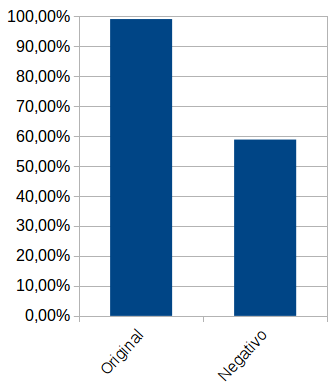
\includegraphics[width=0.3\textwidth]{figures/orig_neg}
		\caption{Porcentaje de acierto de base de datos original y ampliada con negativo.}
		\label{fig.neg-orig}
	\end{center}
\end{figure}
\vspace{20pt}

Para solucionar el problema que acarrea el tener esta gran diferencia únicamente modificando el fondo de la imagen, y puesto que la aplicación no está enfocada a un único tipo de fondo, se opta por aplicar un filtro de bordes que independice la imagen del fondo. Existen varios filtros de bordes que es posible aplicar para solucionar el problema~\cite{fundamentos}.\\

Para desarrollar la comparación entre los diferentes filtros posibles se ha desarrollado un script similar al anterior, en el que se aplicaba el negativo, \textit{create\_edges\_database.py}, que aplicará el filtro de borde seleccionado. Se parte de la base de datos ampliada con el negativo, por lo que no es necesario almacenar la imagen de la que se parte en la base de datos. Será necesario aplicar el filtro, también sobre las bases de datos de entrenamiento y validación, puesto que el objetivo es desarrollar una nueva red neuronal que interprete los bordes. Se obtiene, así, una base de datos de entrenamiento con 48000 muestras, otra de validación con 12000, y una última de test con 20000, a las que se les ha aplicado un determinado filtro de bordes.\\

A continuación se explicarán los tres filtros que han sido evaluados en este proyecto: Canny, Laplaciano y Sobel.

\begin{description}
	\item[Filtro de Canny] \hfill 
	\vspace{5pt}
	\\
	El algoritmo de Canny es un operador desarrollado por John F. Canny en 1986 que utiliza un algoritmo de múltiples etapas para detectar una amplia gama de bordes en imágenes~\cite{4767851}. Para ello utiliza el cálculo de variaciones, una técnica que encuentra la función que optimiza un funcional indicado. En este caso, la función óptima, es definida por la suma de cuatro términos exponenciales, pero se puede aproximar por la primera derivada de una gaussiana. El resultado de aplicar este filtro es siempre una imagen binaria en la que los píxeles únicamente pueden tomar los valores 0 ó 1 (0 ó 255 dependiendo del rango).\\
	\vspace{-10pt}
	\\
	Para aplicar este algoritmo en el código se debe implementar la función proporcionada por \textit{openCV} según~\cite{canny}. En la Figura~\ref{fig.canny} se muestra la aplicación de este filtro para cada dígito mostrado en la Figura~\ref{fig.digitosMNIST}. En la base de datos de test, se van a obtener dos imágenes iguales de cada dígito ya que se está aplicando sobre el original y el negativo el mismo filtro, que por su propio funcionamiento, detecta los mismos bordes en ambos.
	
	\begin{figure}[H]
		\begin{center}
			
\includegraphics[width=0.3\textwidth]{figures/canny}
			\caption{Muestra de dígitos con filtro Canny.}
			\label{fig.canny}
		\end{center}
	\end{figure}
	
	\item[Filtro Laplaciano] \hfill 
	\vspace{5pt}
	\\
	El laplaciano es un operador de segunda derivada que se utiliza con frecuencia en la detección de bordes~\cite{laplacian}. Su fundamento se encuentra en la identificación de un borde cuando se produce un cruce por cero en la segunda derivada obtenida. Este operador posee dos filtros diferentes, uno positivo con el que se obtienen los bordes externos, este es el utilizado en este proyecto, y uno negativo que obtiene los bordes internos de la misma~\cite{laplacian2}. El resultado final será una imagen en escala de grises correspondiente con los bordes de interés.\\
	\vspace{-10pt}
	\\
	La aplicación del filtro es posible gracias a otra función de \textit{openCV}, según~\cite{laplacianOCV}. En la Figura~\ref{fig.laplacian}, se muestra la aplicación de este filtro para cada dígito mostrado en la Figura~\ref{fig.digitosMNIST} y a su negativo. La diferencia entre ambos resultados se debe a que en la imagen original, como se comentó anteriormente, se están obteniendo los bordes externos gracias al operador positivo, pero al aplicarlo en el negativo de la imagen, los correspondientes bordes externos son ahora los internos de la imagen original. Esta diferencia podría perjudicar a la robustez de la red, pues dependiendo de la imagen la diferencia entre ambos podría ser suficiente como para crear confusión.
	\begin{figure}[H]
		\centering
		\subfigure[Original]{
\includegraphics[width=0.3\textwidth]{figures/laplacian-orig}} \hspace{10pt}
		\subfigure[Negativo]{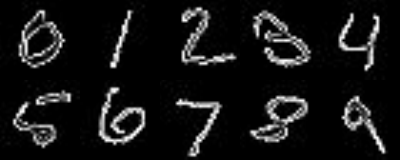
\includegraphics[width=0.3\textwidth]{figures/laplacian-neg}}
		\caption{Muestra de dígitos con filtro Laplaciano.}
		\label{fig.laplacian}
	\end{figure}
	\vspace{-10pt}
	\item[Filtro de Sobel] \hfill 
	\vspace{5pt}
	\\
	Este filtro está formado por dos máscaras de derivadas  que permiten obtener los bordes en una determinada dirección, horizontal y vertical~\cite{sobel}. Para obtener la imagen de bordes final será necesario sumar ambas soluciones,en valor absoluto, obteniendo la imagen de grises con los bordes.\\
	\vspace{-10pt}
	\\
	Para aplicar este filtro primero se debe aplicar cada una de las dos máscaras, horizontal y vertical, gracias a la función de \textit{openCV}~\footnote{http://docs.opencv.org/2.4/doc/tutorials/imgproc/imgtrans/sobel\_derivatives/sobel\_derivatives.html}. Una vez se tienen los bordes en ambas direcciones se suman ambos en valor absoluto y se normaliza a valores entre 0 y 255, obteniendo una imagen de tipo \textit{float} que deberá ser transformada a \textit{uint8}. En la Figura~\ref{fig.sobel} se muestra la aplicación de este filtro para cada dígito mostrado en la Figura~\ref{fig.digitosMNIST}. En este caso, y al igual que en el caso de Canny, se obtiene la misma imagen de bordes en ambas imágenes, pues el filtro no hace distinción entre bordes internos y externos.
	
	\begin{figure}[H]
		\begin{center}
			
\includegraphics[width=0.3\textwidth]{figures/sobel}
			\caption{Muestra de dígitos con filtro de Sobel.}
			\label{fig.sobel}
		\end{center}
	\end{figure}	
\end{description}
\vspace{-10pt}

Una vez obtenidas las diferentes bases de datos con los filtros de bordes aplicados se procede al entrenamiento de tres redes neuronales diferentes, una con cada uno de los filtros, según se explicó en la Sección~\ref{sec.red}. En concreto, únicamente se modificarán las distintas bases de datos empleadas en entrenamiento y evaluación por la obtenida para cada caso.\\

Tras obtener las tres redes neuronales entrenadas será posible comenzar con el test de las mismas según lo explicado en la Sección~\ref{sec.banco}, obteniendo la tasa de acierto para cada uno de ellos, que quedan representados en la Figura~\ref{fig.filtros}. Para ello se ha empleado la base de datos de test ampliada con el negativo aplicando, para cada red, el filtro correspondiente.

\begin{figure}[H]
	\begin{center}
		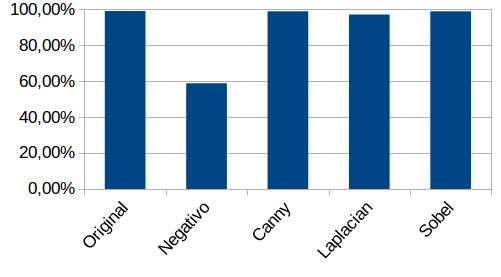
\includegraphics[width=0.5\textwidth]{figures/filtros}
		\caption{Comparación de tasa de acierto con diferentes filtros.}
		\label{fig.filtros}
	\end{center}
\end{figure}

En esta gráfica se puede observar que el uso de imágenes de bordes mejora en gran medida el entrenamiento con un determinado fondo, haciendo la clasificación independiente del mismo. Dentro de los distinto filtros utilizados, todos ellos producen prácticamente el mismo resultado, siendo ligeramente peor el filtro laplaciano por la diferencia entre bordes internos y externos explicada anteriormente. Por todo ello y la preferencia de obtener imágenes en tono de grises, que hagan más robusta la red, se opta por elegir el filtro de Sobel en la aplicación.\\

Para obtener resultados coherentes es fundamental que el preprocesado aplicado a la base de datos en el entrenamiento sea igualmente aplicado a las imágenes antes de introducirlas en la red para la clasificación. Para ello se modificará la función que transforma la imagen obtenida por la cámara en el componente, explicada en la Sección~\ref{sec.camara}, incluyendoo el filtrado de bordes tras eliminar el ruido. En la Figura~\ref{fig.componente2} se puede observar cómo se muestra la imagen final en el componente, aplicando el filtrado indicado.\\

Una vez se ha obtenido una clasificación independiente del fondo de la imagen escogida, dotando a la red de una mayor robustez, se analizarán algunas transformaciones típicas que se pueden dar frecuentemente en un problema real, es decir, se estudiará el efecto de no tener imágenes perfectas sino imágenes ruidosas.

\begin{figure}[H]
	\begin{center}
		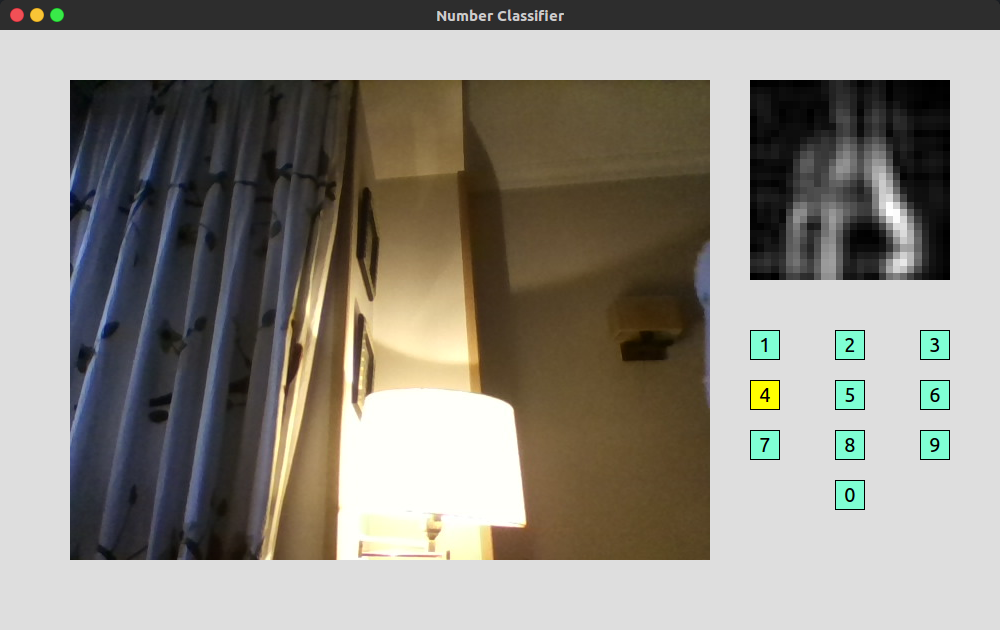
\includegraphics[width=0.5\textwidth]{figures/componente2}
		\caption{Captura del componente clasificador con filtro Sobel.}
		\label{fig.componente2}
	\end{center}
\end{figure}

\subsubsection{Imágenes ruidosas en test}

Al obtener una imagen con la cámara esta puede no estar perfectamente centrada, recta o con un tamaño igual al de la base de datos empleada en el entrenamiento, además de poder incluir ruido introducido por la propia cámara. Esto hará que, al introducir una de estas imágenes en la red, entrenada con imágenes sin ningún tipo de alteración, no se obtenga la precisión deseada.\\

Para la evaluación del ruido sobre la red neuronal, entendiendo por ruido cualquier posible alteración de la imagen, se elaborará una base de datos de test a partir de la que proporciona MNIST de 10000 muestras, incluyendo en ella 6 imágenes con la transformación aplicada y la imagen original para cada muestra, aplicando, por último el filtro de Sobel a cada una. De esta manera se obtiene una base de datos de test con 70000 muestras de bordes ruidosas.\\

Tras aplicar las diferentes transformaciones sobre la base de datos de test se obtendrán diversas bases de datos modificadas que serán introducidas sobre la misma red neuronal, la desarrollada anteriormente con bordes de Sobel, para poder evaluar la robustez de la misma.\\

A continuación se explicarán las distinas transformaciones realizadas, todas ellas con ayuda de las funciones que proporciona \textit{openCV} y cómo afecta cada una a los parámentros que permiten evaluar la red.

\begin{description}
	\item[Rotación] \hfill 
	\vspace{5pt}
	\\
	La rotación consiste en el giro sobre un eje situado en el centro de la imagen,un determinado ángulo establecido por el desarrollador.\\
	\vspace{-10pt}
	\\
	En concreto, en esta aplicación se ha optado por la rotación con un ángulo aleatorio dentro del rango [-20,20] grados. En la Figura~\ref{fig.rotacion} se muestra la aplicación de la rotación para cada dígito mostrado en la Figura~\ref{fig.digitosMNIST}.
	
	\begin{figure}[H]
		\begin{center}
			
\includegraphics[width=0.3\textwidth]{figures/rotacion}
			\caption{Muestra de dígitos rotados.}
			\label{fig.rotacion}
		\end{center}
	\end{figure}
	\vspace{-10pt}
	\item[Traslación] \hfill 
	\vspace{5pt}
	\\
	La traslación de una imagen consiste en desplazar la misma en una determinada dirección y sentido marcados por dos variables \textit{x} e \textit{y}, tomando como referencia el eje central.\\
	\vspace{-10pt}
	\\
	Para la evaluación que es de interés en el proyecto, se ha establecido un rango de desplazamiento horizontal aleatorio de [-4,4] y uno vertical de [-4,2], de tal manera que la imagen del dígito no quede recortada. En la Figura~\ref{fig.traslacion} se muestra la aplicación de la traslación para cada dígito mostrado en la Figura~\ref{fig.digitosMNIST}.
	\begin{figure}[H]
		\begin{center}
			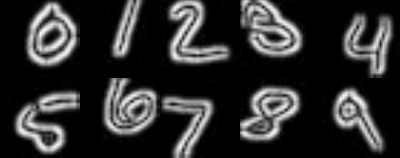
\includegraphics[width=0.3\textwidth]{figures/traslacion}
			\caption{Muestra de dígitos trasladados.}
			\label{fig.traslacion}
		\end{center}
	\end{figure}
	\vspace{-10pt}
	\item[Escalado] \hfill 
	\vspace{5pt}
	\\
	El escalado de una imagen consiste en cambiar el tamaño de la misma estableciendo una proporción, manteniendo el centro de la imagen en el mismo punto.\\
	\vspace{-10pt}
	\\
	Para integrar esta transformación en el estudio realizado se establece un parámetro de proporción aleatorio en el rango [0.5,1.5].\\
	\vspace{-10pt}
	\\
	Tras aplicar el escalado, el resultado es una imagen cuyas dimensiones han variado, aumentando o disminuyendo en función de la proporción. Para introducir las imágenes en la red y obtener resultados adecuados se debe adaptar el tamaño de las mismas al necesario para la red (28x28) sin deformar la imagen. Para ello, si el tamaño de la imagen es mayor, se recortará la misma manteniendo el centro, si por el contrario, el tamaño es menor, se añadirá un borde del mismo color que el fondo de la imagen hasta obtener el tamaño deseado.
	\vspace{10pt}
	\\
	En la Figura~\ref{fig.escalado} se muestra la aplicación de la traslación para cada dígito mostrado en la Figura~\ref{fig.digitosMNIST}.
	\begin{figure}[H]
		\begin{center}
			
\includegraphics[width=0.3\textwidth]{figures/escala}
			\caption{Muestra de dígitos escalados.}
			\label{fig.escalado}
		\end{center}
	\end{figure}
	\item[Ruido] \hfill 
	\vspace{10pt}
	\\
	El ruido de una imagen es una variación aleatoria de la información de brillo o color en la misma. Existen diferentes tipos de ruido con naturalezas distintas que pueden estar producidos por diversas causas como por ejemplo ruido Gaussiano, ruido \textit{Salt\&Pepper} o ruido uniforme.\\
	\vspace{-10pt}
	\\
	La apliación pretende clasificar los dígitos mostrados a una cámara en tiempo real, en donde el ruido más presente es el ruido Gaussiano, por lo que será el empleado para el test. Se aplicará un ruido Gaussiano con  una varianza de 0.02, utilizando, en este caso, una función que proporciona \textit{skimage.util}. En la Figura~\ref{fig.ruido} se muestra la aplicación del ruido para cada dígito mostrado en la Figura~\ref{fig.digitosMNIST}.
	\begin{figure}[H]
		\begin{center}
			
\includegraphics[width=0.3\textwidth]{figures/ruido}
			\caption{Muestra de dígitos con ruido.}
			\label{fig.ruido}
		\end{center}
	\end{figure}
\end{description}

Además de las bases de datos creadas con la transformación única, se elabora una nueva base de datos que contiene una combinación de todas las transformaciones explicadas: escalado, traslación, rotación y ruido, para obtener una evaluación más realista. En esta combinación, a la hora de aplicar la traslación, se tendrá en cuenta el factor de escala aplicado, de tal manera que si es mayor que 1, es decir, la imagen se ha ampliado, el rango de desplazamiento se ve reducido a la mitad en ambas direcciones. De esta manera, el dígito se mantendrá siempre dentro de la imagen, sin verse recortado por ningún lado.\\

En la Figura~\ref{fig.mix} se muestra la aplicación de la traslación para cada dígito mostrado en la Figura~\ref{fig.digitosMNIST}.
\begin{figure}[H]
	\begin{center}
		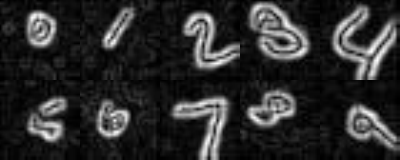
\includegraphics[width=0.3\textwidth]{figures/mix}
		\caption{Muestra de dígitos con mezcla de transformaciones.}
		\label{fig.mix}
	\end{center}
\end{figure}

Una vez se han obtenido las bases de datos que permitan realizar el estudio sobre la robustez de la red, se incluirán en el banco de pruebas explicado en la Sección~\ref{sec.banco} y se obtendrá la tasa de acierto, desglosada por dígitos y de manera global. Estos resultados quedan reflejados en la Figura~\ref{fig.sobelEval}.

\begin{figure}[H]
	\begin{center}
		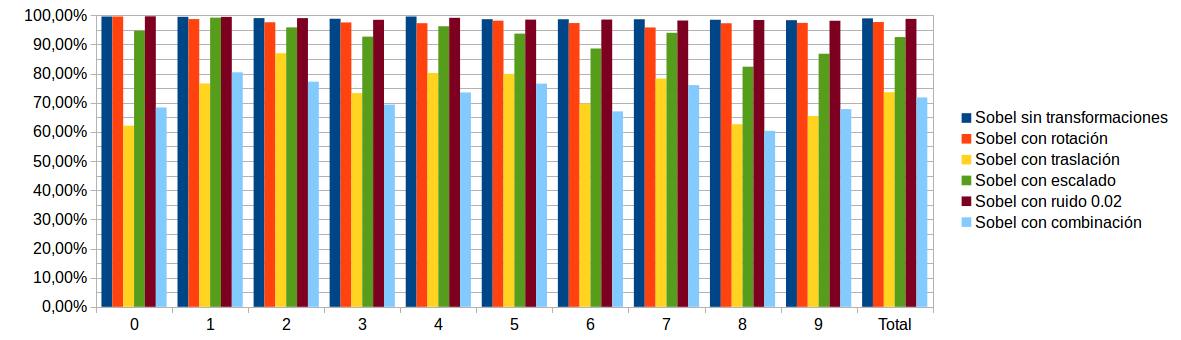
\includegraphics[width=1\textwidth]{figures/sobelev}
		\caption{Evaluación de la red con bases de datos transformadas.}
		\label{fig.sobelEval}
	\end{center}
\end{figure}

Se puede observar que el introducir varias transformaciones sobre la imagen hace que la tasa de acierto disminuya considerablemente, siendo especialmente sensible a la traslación, mientras que el ruido a penas afecta, algo que concuerda con las imágenes mostradas. Estos resultados hacen ver que la red, frente a un escenario real en el que las imágenes no son perfectas, no reaccionaría de la manera que se desearía, existiendo una probabilidad de fallo del 0.3. Por ello, se continuará el estudio elaborando bases de datos de entrenamiento y validación que incluyan estas transformaciones y permitan mejorar la tasa de acierto de la aplicación.

\subsubsection{Imágenes ruidosas en entrenamiento}
Para conseguir desarrollar una red más robusta, según lo analizado las secciones anteriores, se elaborarán nuevas bases de datos de entrenamiento y validación mediante la combinación de las transformaciones explicadas anteriormente. Las nuevas bases de datos serán modificaciones de la utilizada en la red básica, explicada en la Sección~\ref{sec.red}. Para la evaluación de todas las redes creadas se empleará la base de datos de test creada anteriormente, en la que se combinan todas las transformaciones, con 70000 muestras.\\

En primer lugar, se calcula la matriz de confusión de la red entrenada únicamente con las imágenes de bordes de Sobel, que queda reflejada en la Tabla~\ref{tab.matriz1-0}. De esta manera se podrán obtener valores de \textit{precision} y \textit{recall} de la misma y hacer una comparación adecuada de todas las redes.\\
	\begin{table}[H]
		\centering
		\begin{tabular}{|c|l|c|c|c|c|c|c|c|c|c|c|c|}
			\cline{3-13} 
			 \multicolumn{2}{c|}{} & \multicolumn{11}{c|}{\textbf{Real}} \\ \cline{3-13} 
			 \multicolumn{2}{c|}{} & \textbf{0} & \textbf{1} & \textbf{2} &  \textbf{3} & \textbf{4} & \textbf{5} & \textbf{6} & \textbf{7} & \textbf{8} & \textbf{9} & \textbf{Total}\\ \hline
			 \multirow{10}{0.5cm}{\rotatebox{90}{\textbf{Predicción}}}& \textbf{0} &  \cellcolor{lightgray}4691 & 191 & 82 & 90 & 118 & 83 & 173 & 45 & 163 & 192 & 5828\\ \cline{2-13}
			 & \textbf{1} & 76 & \cellcolor{lightgray}6391 & 119 & 65 & 213 & 22 & 209 & 212 & 246 & 142 & 7695\\ \cline{2-13}
			 & \textbf{2} & 188 & 98 & \cellcolor{lightgray}5578 & 462 & 232 & 131 & 121 & 683 & 276 & 229 & 7998\\ \cline{2-13}
			 & \textbf{3} & 43 & 30 & 443 & \cellcolor{lightgray}4904 & 270 & 201 & 48 & 275 & 243 & 311 & 6768\\ \cline{2-13}
			 & \textbf{4} & 158 & 415 & 291 & 145 & \cellcolor{lightgray}5055 & 117 & 720 & 37 & 320 & 381 & 7639\\ \cline{2-13}
			 & \textbf{5} & 96 & 72 & 65 & 633 & 107 & \cellcolor{lightgray}4780 & 234 & 112 & 323 & 243 & 6665\\ \cline{2-13}
			 & \textbf{6} & 472 & 234 & 86 & 49 & 130 & 216 & \cellcolor{lightgray}4497 & 15 & 326 & 91 & 6116\\ \cline{2-13}
			 & \textbf{7} & 57 & 416 & 265 & 255 & 244 & 105 & 19 & \cellcolor{lightgray}5473 & 235 & 488 & 7557\\ \cline{2-13}
			 & \textbf{8} & 138 & 80 & 131 & 139 & 139 & 129 & 182 & 84 & \cellcolor{lightgray}4116 & 194 & 5332\\ \cline{2-13}
			 & \textbf{9} & 941 & 18 & 164 & 328 & 366 & 460 & 503 & 260 & 570 & \cellcolor{lightgray}4792 & 8402\\ \cline{2-13} 
			 & \textbf{Total} & 6860 & 7945 & 7224 & 7070 & 6874 & 6244 & 6706 & 7196 & 6818 & 7063 & 70000\\ \hline
		\end{tabular}
		\caption{Matriz de confusión red 1-0.}
		\label{tab.matriz1-0}
	\end{table}
	
Tras obtener la evaluación de la red basica, se procede a la modificación de la misma y su posterior evaluación, variando el número de imágenes transformadas que se utilizan, así como la inclusión o no de la imagen original. Para esta tarea, se partirá de la base de datos de entrenamiento modificada de la misma manera que se modificó la de test en la sección anterior, obteniendo 6 transformaciones y la imagen original. Tras evaluar los resultados, se irá reduciendo el número de imágenes, para evaluar el impacto y conseguir una base de datos que proporcione buenos resultados disminuyendo la complejidad de cómputo.
\vspace{5pt}

\begin{description}
	\item[Base de datos 1-6] \hfill 
	\vspace{5pt}
	\\
	Para elaborar esta base de datos se utilizan 6 imágenes transformadas y la imagen original con la aplicación de los filtros de Sobel. De esta forma se obtiene una base de datos de entrenamiento de 336000 muestras y una de validación de 84000 muestras.\\
	\vspace{-10pt}
	\\
	Con estas bases de datos se entrena una nueva red y se calcula la matriz de confusión, mostrada en la Tabla~\ref{tab.matriz1-6}.
	\begin{table}[H]
		\centering
		\begin{tabular}{|c|l|c|c|c|c|c|c|c|c|c|c|c|}
			\cline{3-13}  
			\multicolumn{2}{c|}{} & \multicolumn{11}{c|}{\textbf{Real}} \\ \cline{3-13} 
			\multicolumn{2}{c|}{} & \textbf{0} & \textbf{1} & \textbf{2} &  \textbf{3} & \textbf{4} & \textbf{5} & \textbf{6} & \textbf{7} & \textbf{8} & \textbf{9} & \textbf{Total}\\ \hline
			\multirow{10}{0.5cm}{\rotatebox{90}{\textbf{Predicción}}}& \textbf{0} & \cellcolor{lightgray}6770 & 13 & 24 & 13 & 7 & 35 & 74 & 2 & 161 & 40 & 7139\\ \cline{2-13}
			& \textbf{1} & 1 & \cellcolor{lightgray}7868 & 26 & 15 & 13 & 15 & 25 & 43 & 11 & 12 & 8029\\ \cline{2-13}
			& \textbf{2} & 13 & 16 & \cellcolor{lightgray}6890 & 125 & 5 & 10 & 6 & 62 & 47 & 8 & 7182\\ \cline{2-13}
			& \textbf{3} & 1 & 3 & 9 & \cellcolor{lightgray}6567 & 0 & 66 & 0 & 3 & 9 & 8 & 6666\\ \cline{2-13}
			& \textbf{4} & 18 & 3 & 53 & 13 & \cellcolor{lightgray}6610 & 24 & 52 & 9 & 74 & 71 & 6927\\ \cline{2-13}
			& \textbf{5} & 3 & 0 & 1 & 95 & 0 & \cellcolor{lightgray}5820 & 16 & 2 & 17 & 5 &5959\\ \cline{2-13}
			& \textbf{6} & 25 & 10 & 7 & 3 & 10 & 123 & \cellcolor{lightgray}6519 & 0 & 71 & 2 & 6770\\ \cline{2-13}
			& \textbf{7} & 13 & 25 & 170 & 119 & 32 & 17 & 1 & \cellcolor{lightgray}7030 & 43 & 108 & 7558\\ \cline{2-13}
			& \textbf{8} & 4 & 7 & 31 & 54 & 7 & 67 & 9 & 8 & \cellcolor{lightgray}6234 & 12 & 6433\\ \cline{2-13}
			& \textbf{9} & 12 & 0 & 13 & 66 & 190 & 67 & 4 & 37 & 151 & \cellcolor{lightgray}6797 & 7337\\ \cline{2-13}
			& \textbf{Total} & 6860 & 7945 & 7224 & 7070 & 6874 & 6244 & 6706 & 7196 & 6818 & 7063 & 70000\\ \hline
		\end{tabular}
		\caption{Matriz de confusión red 1-6.}
		\label{tab.matriz1-6}
	\end{table}
	\item[Base de datos 1-1] \hfill 
	\vspace{5pt}
	\\
	En este caso se reducirá el número de imágenes transformadas para comprobar la importancia de las mismas en el aprendizaje. El objetivo es tratar de reducir el número de muestras en la base de datos de entrenamiento y validación para disminuir la carga computacional manteniendo la máxima precisión posible.\\
	\vspace{-10pt}
	\\
	Para lograr el objetivo se incluirá en la base de datos de entrenamiento y de validación una única imagen transformada y la imagen original, obteniendo un total de 96000 muestras en la base de datos de entrenamiento y 24000 en la de validación.\\
	\vspace{-10pt}
	\\
	Tras obtener las bases de datos se entrenará una nueva red de la que se obtendrá de nuevo la matriz de confusión, representada en la Tabla~\ref{tab.matriz1-1}.
	\begin{table}[H]
		\centering
		\begin{tabular}{|c|l|c|c|c|c|c|c|c|c|c|c|c|}
			\cline{3-13} 
			\multicolumn{2}{c|}{} & \multicolumn{11}{c|}{\textbf{Real}} \\ \cline{3-13} 
			\multicolumn{2}{c|}{} & \textbf{0} & \textbf{1} & \textbf{2} &  \textbf{3} & \textbf{4} & \textbf{5} & \textbf{6} & \textbf{7} & \textbf{8} & \textbf{9} & \textbf{Total}\\ \hline
			\multirow{10}{0.5cm}{\rotatebox{90}{\textbf{Predicción}}}& \textbf{0} & \cellcolor{lightgray}6637 & 6 & 29 & 8 & 9 & 11 & 36 & 4 & 56 & 39 & 6835\\ \cline{2-13}
			& \textbf{1} & 3 & \cellcolor{lightgray}7821 & 29 & 9 & 16 & 4 & 18 & 35 & 5 & 16 & 7956\\ \cline{2-13}
			& \textbf{2} & 13 & 10 & \cellcolor{lightgray}6747 & 45 & 21 & 2 & 8 & 107 & 37 & 12 & 7002\\ \cline{2-13}
			& \textbf{3} & 8 & 16 & 117 & \cellcolor{lightgray}6703 & 2 & 97 & 4 & 35 & 66 & 42 & 7090\\ \cline{2-13}
			& \textbf{4} & 2 & 4 & 45 & 10 & \cellcolor{lightgray}6576 & 9 & 41 & 33 & 38 & 164 & 6922\\ \cline{2-13}
			& \textbf{5} & 26 & 4 & 27 & 152 & 18 & \cellcolor{lightgray}5989 & 80 & 28 & 84 & 91 & 6499\\ \cline{2-13}
			& \textbf{6} & 116 & 31 & 10 & 2 & 66 & 51 & \cellcolor{lightgray}6474 & 0 & 82 & 10 & 6842\\ \cline{2-13}
			& \textbf{7} & 19 & 30 & 135 & 58 & 29 & 12 & 0 & \cellcolor{lightgray}6873 & 27 & 89 & 7272\\ \cline{2-13}
			& \textbf{8} & 23 & 21 & 68 & 70 & 35 & 54 & 41 & 20 & \cellcolor{lightgray}6345 & 66 & 6743\\ \cline{2-13}
			& \textbf{9} & 13 & 2 & 17 & 13 & 102 & 15 & 4 & 61 & 78 & \cellcolor{lightgray}6534 & 6839\\ \cline{2-13}
			& \textbf{Total} & 6860 & 7945 & 7224 & 7070 & 6874 & 6244 & 6706 & 7196 & 6818 & 7063 & 70000\\ \hline
		\end{tabular}
		\caption{Matriz de confusión red 1-1.}
		\label{tab.matriz1-1}
	\end{table}
	\item[Base de datos 0-6] \hfill 
	\vspace{10pt}
	\\
	La siguiente reducción consiste en mantener las 6 transformaciones de la imagen en cada muestra pero no incluir la original. De esta manera se podrá establecer una conclusión sobre la importancia de la imagen original en la mejora del aprendizaje.\\
	\vspace{-10pt}
	\\
	En esta ocasión se tendrá una base de datos de entrenamiento con 288000 muestras y una de validación con 72000. Al igual que en los casos anteriores se entrenará una nueva red y se obtendrá su matriz de confusión, respresentada en la Tabla~\ref{tab.matriz0-6}.
	\begin{table}[H]
		\centering
		\begin{tabular}{|c|l|c|c|c|c|c|c|c|c|c|c|c|}
			\cline{3-13} 
			\multicolumn{2}{c|}{} & \multicolumn{11}{c|}{\textbf{Real}} \\ \cline{3-13} 
			\multicolumn{2}{c|}{} & \textbf{0} & \textbf{1} & \textbf{2} &  \textbf{3} & \textbf{4} & \textbf{5} & \textbf{6} & \textbf{7} & \textbf{8} & \textbf{9} & \textbf{Total}\\ \hline
			\multirow{10}{0.5cm}{\rotatebox{90}{\textbf{Predicción}}}& \textbf{0} & \cellcolor{lightgray}6639 & 0 & 23 & 8 & 5 & 12 & 16 & 1 & 41 & 16 & 6761\\ \cline{2-13}
			& \textbf{1} & 4 & \cellcolor{lightgray}7853 & 12 & 8 & 14 & 1 & 11 & 62 & 2 & 13 & 7980\\ \cline{2-13}
			& \textbf{2} & 14 & 18 & \cellcolor{lightgray}7022 & 78 & 31 & 6 & 13 & 133 & 58 & 6 & 7379\\ \cline{2-13}
			& \textbf{3} & 1 & 15 & 29 & \cellcolor{lightgray}6797 & 1 & 69 & 4 & 29 & 32 & 27 & 7004\\ \cline{2-13}
			& \textbf{4} & 12 & 5 & 21 & 1 & \cellcolor{lightgray}6675 & 3 & 24 & 24 & 40 & 149 & 6954\\ \cline{2-13}
			& \textbf{5} & 19 & 3 & 4 & 90 & 7 & \cellcolor{lightgray}6065 & 57 & 7 & 91 & 50 & 6393\\ \cline{2-13}
			& \textbf{6} & 117 & 23 & 9 & 1 & 19 & 46 & \cellcolor{lightgray}6545 & 0 & 62 & 7 & 6829\\ \cline{2-13}
			& \textbf{7} & 16 & 13 & 58 & 43 & 12 & 6 & 0 & \cellcolor{lightgray}6859 & 24 & 65 & 7096\\ \cline{2-13}
			& \textbf{8} & 30 & 13 & 36 & 34 & 15 & 27 & 36 & 10 & \cellcolor{lightgray}6399 & 30 & 6630\\ \cline{2-13}
			& \textbf{9} & 8 & 2 & 10 & 10 & 95 & 9 & 0 & 71 & 69 & \cellcolor{lightgray}6700 & 6974\\ \cline{2-13}
			& \textbf{Total} & 6860 & 7945 & 7224 & 7070 & 6874 & 6244 & 6706 & 7196 & 6818 & 7063 & 70000\\ \hline
		\end{tabular}
		\caption{Matriz de confusión red .}
		\label{tab.matriz}
	\end{table}
	\item[Base de datos 0-1] \hfill 
	\vspace{10pt}
	\\
	Finalmente, visto que los resultados de la reducción de muestras explicadas anteriormente resultan bastante satisfactorios, se reduce el número de imágenes transformadas utilizadas y no se incluye la imagen original, obteniendo una base de datos de entrenamiento de 48000 muestras y de validación de 12000.\\
	\vspace{-10pt}
	\\
	Con esta nueva base de datos se entrena una nueva red y se obtiene su matriz de confusión, reflejada en la Tabla~\ref{tab.matriz0-1}.
	\begin{table}[H]
		\centering
		\begin{tabular}{|c|l|c|c|c|c|c|c|c|c|c|c|c|}
			\cline{3-13} 
			\multicolumn{2}{c|}{} & \multicolumn{11}{c|}{\textbf{Real}} \\ \cline{3-13} 
			\multicolumn{2}{c|}{} & \textbf{0} & \textbf{1} & \textbf{2} &  \textbf{3} & \textbf{4} & \textbf{5} & \textbf{6} & \textbf{7} & \textbf{8} & \textbf{9} & \textbf{Total}\\ \hline
			\multirow{10}{0.5cm}{\rotatebox{90}{\textbf{Predicción}}}& \textbf{0} & \cellcolor{lightgray}6728 & 4 & 31 & 10 & 11 & 18 & 63 & 6 & 66 & 41 & 6978\\ \cline{2-13}
			& \textbf{1} & 2 & \cellcolor{lightgray}7854 & 32 & 8 & 26 & 7 & 27 & 72 & 9 & 20 & 8057\\ \cline{2-13}
			& \textbf{2} & 10 & 22 & \cellcolor{lightgray}6873 & 79 & 27 & 11 & 15 & 145 & 59 & 13 & 7254\\ \cline{2-13}
			& \textbf{3} & 5 & 15 & 51 & \cellcolor{lightgray}6661 & 6 & 79 & 5 & 38 & 30 & 27 & 6917\\ \cline{2-13}
			& \textbf{4} & 1 & 2 & 39 & 6 & \cellcolor{lightgray}6348 & 2 & 25 & 16 & 31 & 65 & 6535\\ \cline{2-13}
			& \textbf{5} & 15 & 1 & 7 & 137 & 6 & \cellcolor{lightgray}5964 & 64 & 11 & 61 & 43 & 6309\\ \cline{2-13}
			& \textbf{6} & 45 & 16 & 12 & 3 & 38 & 61 & \cellcolor{lightgray}6462 & 0 & 60 & 8 & 6705\\ \cline{2-13}
			& \textbf{7} & 14 & 18 & 93 & 55 & 33 & 10 & 0 & \cellcolor{lightgray}6833 & 25 & 86 & 7167\\ \cline{2-13}
			& \textbf{8} & 26 & 12 & 73 & 88 & 62 & 56 & 40 & 12 & \cellcolor{lightgray}6391 & 52 & 6812\\ \cline{2-13}
			& \textbf{9} & 14 & 1 & 13 & 23 & 317 & 36 & 5 & 63 & 86 & \cellcolor{lightgray}6708 & 7266\\ \cline{2-13}
			& \textbf{Total} & 6860 & 7945 & 7224 & 7070 & 6874 & 6244 & 6706 & 7196 & 6818 & 7063 & 70000\\ \hline
		\end{tabular}
		\caption{Matriz de confusión red .}
		\label{tab.matriz0-1}
	\end{table}
\end{description}

Una vez se han obtenido las matrices de confusión de cada una de las redes neuronales entrenadas, se pueden establecer algunas conclusiones a simple vista. En primer lugar, es clara la mejora al entrenar introduciendo alguna imagen ruidosa, ya que, si se observan los valores de la diagonal, correspondiente con los dígitos correctamente clasificados, éstos son superiores al introducir el ruido en el entrenamiento. Además, entrenar introduciendo un mayor número de imágenes de ruido, aparentemente, no aporta gran información a la red, siendo los resultados muy similares en las redes 1-6 y 1-1. Finalmente, introducir la imagen original en el entrenamiento, tampoco aporta información fundamental, pues los resultados obtenidos con la red 1-1 y la red 0-1 son muy similares, al igual que ocurre con las redes 1-6 y 0-6.\\

Para poder establecer conclusiones más firmes, se calculan el \textit{precision} y \textit{recall} de cada una de las redes, con ayuda de la matriz de confusión obtenida según lo explicado en la Sección~\ref{sec.banco}. Estos resultados quedan reflejados en la Figura~\ref{fig.precision-recall}.
\begin{figure}[H]
	\centering
	\subfigure[]{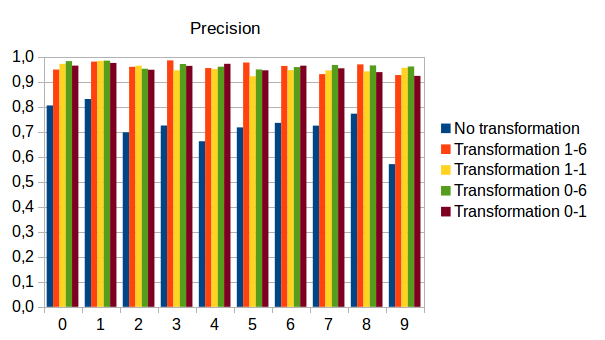
\includegraphics[width=0.4\textwidth]{figures/precision}}
	\subfigure[]{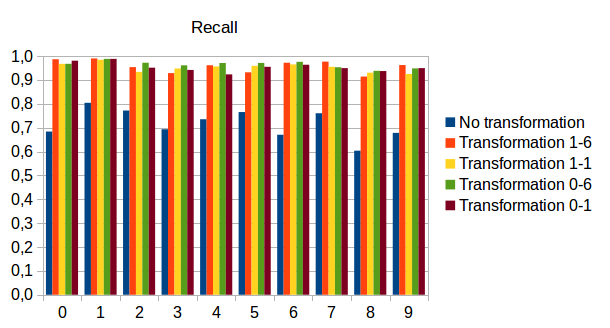
\includegraphics[width=0.4\textwidth]{figures/recall}}
	\caption{Resultados de parámetros de evaluación: (a) \textit{Precision}, (b) \textit{Recall}}
		\label{fig.precision-recall}
\end{figure}
Los resultados obtenidos confirman las conclusiones que se alcanzaron con anterioridad. Existe una clara mejora al introducir imágenes ruidosas en el entrenamiento, una única imagen ruidosa aporta suficiente información y la inclusión de la imagen original no aporta gran información para el entrenamiento.\\

Tras mejorar la red en cuanto a términos de precisión con el cambio en las bases de datos, se analizará la posibilidad de reducir el número de iteraciones para disminuir la carga de cómputo en el entrenamiento de la red.\\

\subsection{Número de iteraciones}
Hasta ahora, se había fijado el número de iteraciones que se realizan en el entrenamiento de la red en un valor de 10000, siendo la iteración, según lo explicado en la Sección~\ref{sec.caffe}, el paso por un \textit{batch}. Sin embargo, este número de iteraciones no tiene por qué ser el más idóneo para la aplicación.\\

Durante el entrenamiento de una red neuronal el aprendizaje es progresivo, de esta manera, la red obtenida en la iteración \textit{n+1} es mejor que la obtenida en la iteración \textit{n}. Ésto se cumple hasta un cierto punto. Existe un momento durante el entrenamiento de la red en el que la mejora entre iteraciones consecutivas es prácticamente nula, pudiéndose producir, incluso, un deterioro en la red. Este deterioro de la red es conocido como sobreaprendizaje, producido por la excesiva focalización en las muestras proporcionadas en el entrenamiento empeorando la generalización.\\

Como se comentó en la Sección~\ref{sec.red}, Caffe permite obtener durante el entrenamiento un archivo \textit{log} en el que se plasman los datos de \textit{accuracy} calculados cada cierto número de iteraciones. Estos resultados han sido recogidos para cada una de las redes explicadas en la sección anterior, obteniendo una comparativa, mostrada en la Figura~\ref{fig.iteraciones}, que permita seleccionar la red más adecuada para la aplicación.
\begin{figure}[H]
	\begin{center}
		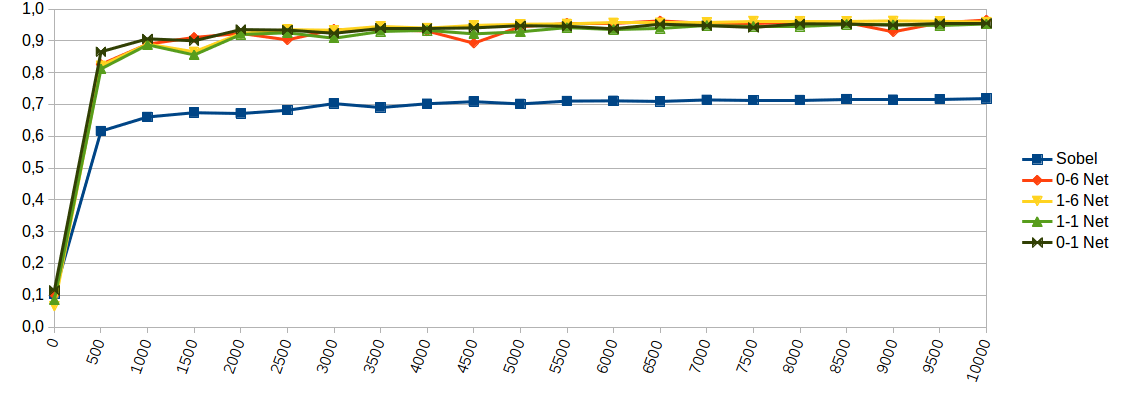
\includegraphics[width=0.7\textwidth]{figures/iteraciones}
		\caption{Red básica LeNet MNIST.}
		\label{fig.iteraciones}
	\end{center}
\end{figure}
En esta figura se puede comprobar que, además de la mejora mencionada anteriormente al introducir imágenes de ruido en el entrenamiento, la estabilidad de la red se alcanza mucho antes de las 10000 iteraciones marcadas.\\

Por todo lo mencionado anteriormente, se decide escoger la red entrenada con la base de datos 0-1 parando en la iteración 5000, obteniendo buenos resultados en cuanto a la precisión de la red y disminuyendo consideráblemente la carga computacional, pues se reduce más de la mitad el número de iteraciones de entrenamiento de la red y se mantiene el número de muestras de las bases de datos de entrenamiento y validación, aunque estas hayan sido modificadas.\\

\section{Experimentos}
Tras todo el análisis realizado anteriormente se ha obtenido una red neuronal más robusta que permite una mejor clasificación en tiempo real de los dígitos mostrados a la cámara. Con todo lo estudiado en puntos anteriores se realiza una comparación entre la primera red básica que se desarrolló y la red a la que se le han aplicado las variaciones precisas.\\

En primer lugar se prueba la aplicación con un dígito cuyo fondo es negro, tal y como se entrenó en la primera red desarrollada. Los resultados de este experimento quedan reflejados en la Figura~\ref{fig.experimento1}.

\begin{figure}[H]
	\centering
	\subfigure[Red básica]{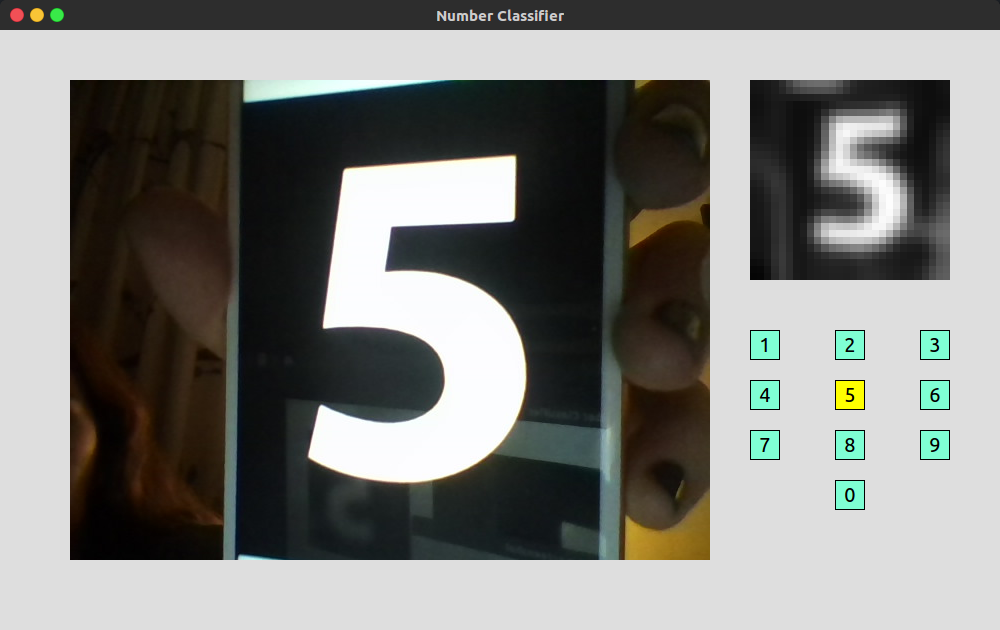
\includegraphics[width=0.4\textwidth]{figures/exp_basica1}} \hspace{5pt}
	\subfigure[Red robusta]{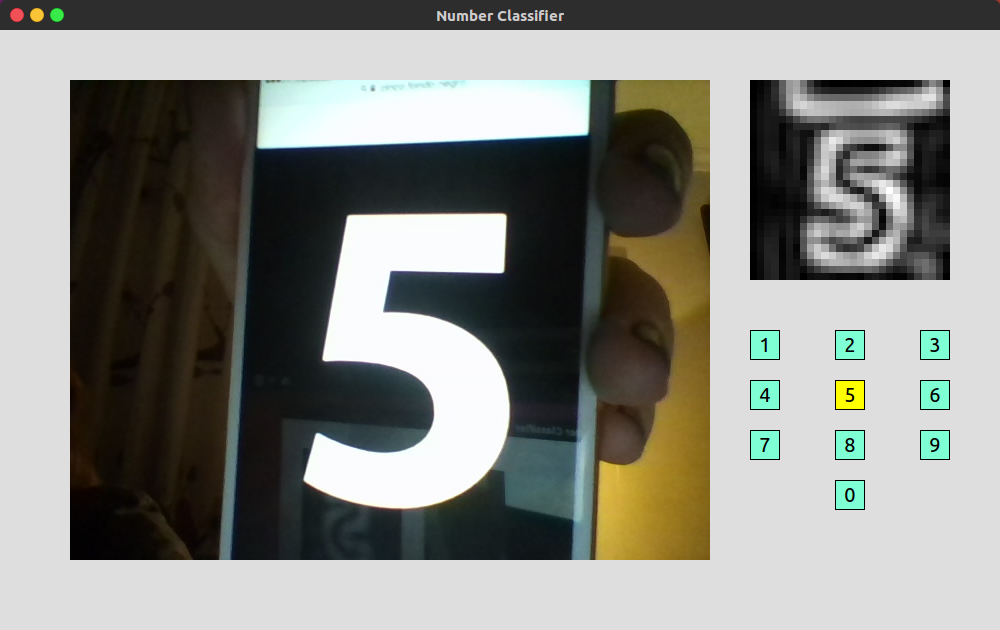
\includegraphics[width=0.4\textwidth]{figures/exp_robusta1}}
	\caption{Evaluación de la aplicación con imagen de fondo negro.}
	\label{fig.experimento1}
\end{figure}

Tras evaluar un ejemplo completamente limpio se pone a prueba la aplicación con una imagen más complicada para la misma, variando su fondo y no siendo tan perfecto. Esta prueba queda reflejada en la Figura~\ref{fig.experimento}, donde se expone un ejemplo con el que se comprueba cómo un dígito que con la red básica que se desarrolló en primer lugar no lograba ser identificado, pues no cumplia con todas las características que la red exigía para ser más precisa, sí es posible su clasificación tras mejorar la red entrenada según lo estudiado en los puntos anteriores. 

\begin{figure}[H]
	\centering
	\subfigure[Red básica]{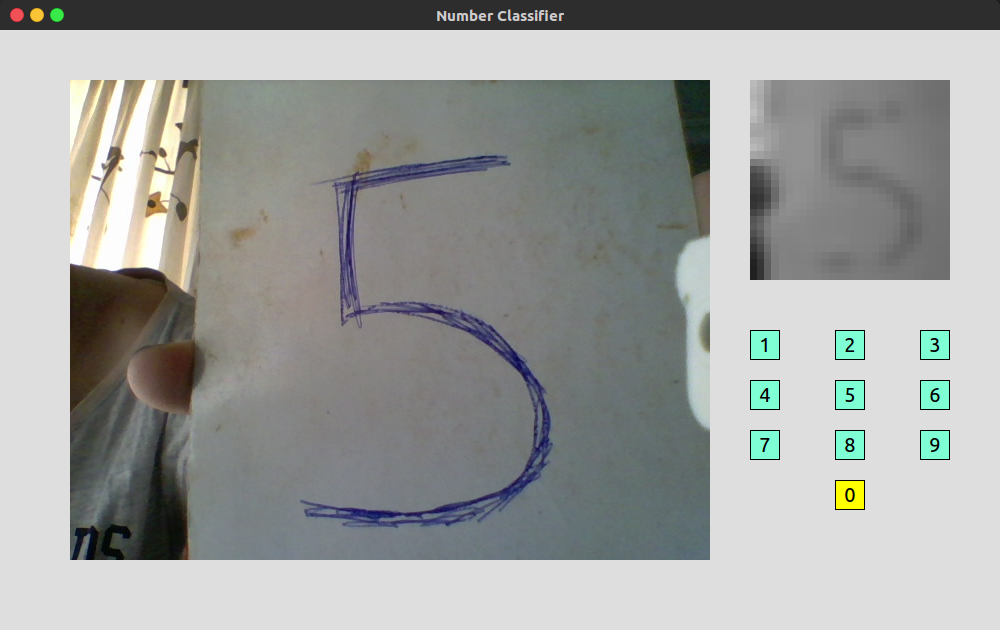
\includegraphics[width=0.4\textwidth]{figures/exp_basica}} \hspace{5pt}
	\subfigure[Red robusta]{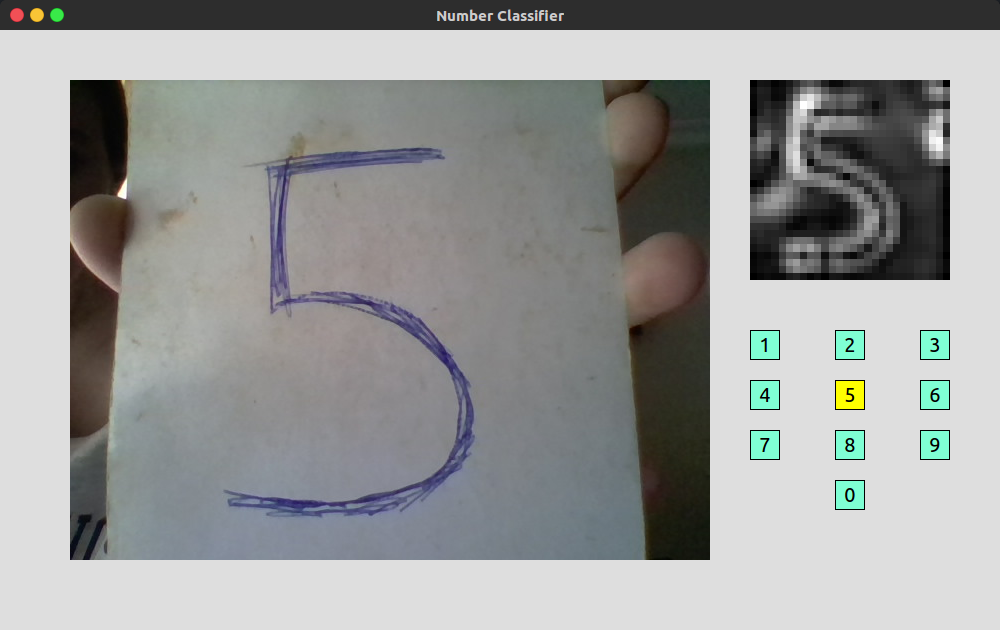
\includegraphics[width=0.4\textwidth]{figures/exp_robusta}}
	\caption{Evaluación de la aplicación con diferentes redes.}
	\label{fig.experimento}
\end{figure}

Para realizar los experimentos anteriores se ha tomado como "Red básica", la explicada en la Sección~\ref{sec.red}, en cuyo entrenamiento únicamente se disponía de imágenes con fondo negro y el dígito en blanco. Como era de esperar, y se demostró en la Sección~\ref{sec.bordes}, al mostrar a la cámara un dígito con el fondo blanco la red hace una clasificación errónea. En el caso de la "Red robusta", se ha seleccionado la red que se concluyó tras la Sección~\ref{sec.mod_bbdd}, una red entrenada con imágenes transformadas a las que se les ha aplicado el filtro de bordes Sobel iterando un total de 5000 veces, permitiendo independizar la imagen del fondo y que la imagen obtenida por la cámara no sea tan perfecta. Con esta nueva red la aplicación sí consigue clasificar correctamente el mismo dígito mostrado a la cámara.\\

La aplicación desarrollada es una muestra sencilla de herramienta para la clasificación de imágenes con mediante técnicas de aprendizaje profundo. Este ejemplo abre una nueva puerta para abarcar nuevos problemas de clasificación más complejos, con bases de datos más completas, que permitan solucionar problemas de interés para el ser humano.
\lhead[]{CAPÍTULO \thechapter. DETECCIÓN}
\chapter{Detección con Aprendizaje Profundo}\label{cap.deteccion}
En este capítulo se realizará una primera aproximación al problema de la detección mediante el aprendizaje profundo utilizando la misma plataforma que se ha estado empleando hasta el momento, Caffe. Para ello se ha utilizado la rama \textit{\acrfull{ssd}}~\cite{liu2016ssd}de la misma, que, además de permitir el entrenamiento de modelos para la detección de diferentes objetos en función de la base de datos utilizada, ofrece varios modelos que ya han sido entrenados para facilitar esta tarea.\\

El método utilizado, \acrshort{ssd}, es diseñado para detectar objetos en imágenes utilizando una única red neuronal profunda. El enfoque \acrshort{ssd} se basa en una red convolucional \textit{feed-forward} que produce una colección de tamaño fijo de cajas delimitadoras(\textit{bounding boxes}) y puntuaciones para la presencia de instancias de clase de objetos en esas cajas, seguido de un paso de supresión no máxima para producir las detecciones finales. Las primeras capas de red se basan en una arquitectura estándar utilizada para la clasificación de imágenes de alta calidad (truncada antes de cualquier clasificación), similar a la explicada en el Capítulo~\ref{cap.clasificacion}. Posteriormente se añade una estructura auxiliar a la red para producir las detecciones, teniendo en cuenta una serie de características clave:
\begin{itemize}
	\item \textbf{Mapas de características de múltiples escalas para detección.} Se añaden capas de características convolucionales al final de la red base truncada, cuyyo tamaño disminuye progresivamente, permitiendo predicciones de detecciones a múltiple escalas. El modelo convolucional para la predicción de las detecciones es diferente para cada capa característica.
	\vspace{10pt}
	\item \textbf{Predictores convolucionales para la detección.} Cada capa de característica añadida puede producir un conjunto fijo de predicciones de detección usando un conjunto de filtros convolucionales, que son indicados en la parte superior de la arquitectura de red \acrshort{ssd}.
	\item \textbf{Cajas por defecto y relaciones de aspecto.} Se asocia un conjunto de cajas delimitadoras predeterminadas con cada celda de mapa de carcaterísticas, para varios mapas de características en la parte superior de la red. Las cajas por defecto anidan el mapa de características de una manera convolucional, de modo que la posición de cada caja con respecto a su celda correspondiente es fija. En cada celda de mapa de características, se predicen los desplazamientos relativos a las formas de cajas predeterminadas en la celda, así como las puntuaciones por clase que indican la presencia de una instancia de clase en cada uno de esas cajas.
\end{itemize}

En la Figura~\ref{fig.ssd} se muestra un resumen del funcionamiento de este modelo. \acrshort{ssd} sólo necesita una imagen de entrada y cajas de verdad para cada objeto durante el entrenamiento. De forma convolucional, se evalua un conjunto pequeño de cajas predeterminadas de diferentes relaciones de aspecto en cada ubicación en varios mapas de características con diferentes escalas (por ejemplo, $8\times8$ en~(b) y $4\times4$ en~(c)). Para cada caja predeterminada se predice tanto los desplazamientos de forma como las confidencias para todas las categorías de objetos (($c_1, c_2, ... , c_p)$). En el momento del entrenamiento, primero se coincide con estas cajas por defecto las casillas de verdad.

\begin{figure}[H]
	\begin{center}
		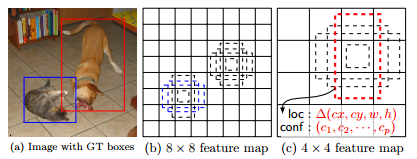
\includegraphics[width=0.6\textwidth]{figures/ssd}
		\caption{Modelo \acrshort{ssd}. Imagen obtenida de~\cite{2015arXiv151202325L}}
		\label{fig.ssd}
	\end{center}
\end{figure} 

Durante el entrenamiento es necesario determinar qué casillas por defecto corresponden a una detección de verdad y entrenar la red en consecuencia. Se comienza haciendo coincidir cada caja de verdad con la caja predeterminada con la mejor superposición de \textit{Jaccard}, un estadístico utilizado para comparar la similitud y diversidad de conjuntos de muestras. 
Esto simplifica el problema de aprendizaje, permitiendo a la red predecir puntuaciones altas para múltiples cajas por defecto superpuestas en lugar de requerir que elija sólo la que tenga superposición máxima. Tras el paso de la coincidencia, la mayoría de las cajas predeterminadas son negativas, especialmente cuando el número de cajas predeterminadas posibles es grande, introduciendo un desequilibrio significativo entre los ejemplos de entrenamiento positivos y negativos. Poe ello es necesario realizar una minería negativa dura, de tal manera que, en lugar de usar todos los ejemplos negativos, se clasifican usando la pérdida de confianza más alta para cada caja predeterminada y se seleccionan los más altos para que la relación entre los negativos y los positivos sea como mucho 3:1, conduciendo a una optimización más rápida y un entrenamiento más estable. Pr último, para hacer que el modelo sea más robusto a los diferentes tamaños y formas de los objetos de entrada, cada imagen de entrenamiento se muestreará aleatoriamente mediante el uso de toda la imagen de entrada original, el muestreo de un parche de modo que la superposición mínima de jaccard con los objetos sea de 0.1, 0.3,
0.5, 0.7 o 0.9, o el muestreo al azar un parche.\\

Una vez entendido el funcionamiento de las redes \acrshort{ssd}, cuya información ha sido obtenida de~\cite{2015arXiv151202325L}, se pasará al uso de algunos ejemplos de las mismas, proporcionadas por la propia rama de la plataforma Caffe. El motivo del uso de estos modelos ya entrenados viene dado por la alta capacidad de cómputo necesaria para entrenar este tipo de redes y la el tiempo que implica el entrenamiento. En concreto se analizarán algunas imágenes con dos de las redes \acrshort{ssd} que se proporcionan:
\begin{itemize}
	\item \textbf{VOC0712-SSD300x300.} Este modelo ha sido entrenado con las bases de datos \textit{Pascal VOC} de los años 2007~\cite{pascal-voc-2007} y 2012~\cite{pascal-voc-2012}, explicadas en la Sección~\ref{sec.voc}. Se utilizan imágenes de 300x300 y la red formada en la iteración 120000.
	\item \textbf{COCO-SSD300x300} Este modelo ha sido entrenado con las bases de datos \acrshort{coco}, explicadas en la Sección~\ref{sec.coco}. Se utilizan imágenes de 300x300 y la red formada en la iteración 120000.
\end{itemize}

Estos modelos proporcionados por la rama \acrshort{ssd} de Caffe pueden ser descargados de su repositorio \textit{Git Hub}~\footnote{https://github.com/weiliu89/caffe/tree/ssd} y utilizados para desarrollar la aplicación que sea de interés.\\

Al obtener los modelos se encuentra una carpeta con una serie de archivos que permiten comprobar la estructura de la red, el solucionador o el propio modelo entrenado entre otros. La aplicación de interés, se centra en el uso de tres de los archivos proporcionados:
\begin{itemize}
	\item \textbf{\textit{labelmap\_voc.prototxt}}, contiene la estructura de las diferentes etiquetas que pueden ser asignadas.
	\item \textbf{\textit{deploy.prototxt}}, contiene la estructura del modelo entrenado.
	\item \textbf{\textit{model\_iter\_niter.caffemodel}}, contiene los pesos del modelo, \textit{model}, entrenado hasta la iteración \textit{niter}.
\end{itemize}

Una vez se dispone del modelo entrenado que se quiere utilizar se ha desarrollado un pequeño \textit{script} en Python, \textit{image\_detection.py} que permite introducir una determinada imagen, realizar la detección sobre ella con el modelo escogido, y obtener una nueva imágen en la que se marcan las detecciones realizadas según un determinado criterio. Para ello se ha utilizado como guía el ejemplo proporcionado en el mismo \textit{Git Hub} de la rama~\footnote{https://github.com/weiliu89/caffe/blob/ssd/examples/ssd\_detect.ipynb}\\

Para poder realizar la detección con el \textit{script} mencionado, lo primero que se debe hacer es indicar la red \acrshort{ssd} que se empleará. Para ello se utilizan unas líneas similares a las empleadas en la Sección~\ref{sec.camara}, con alguna variación para adaptarla al problema de la detección, según se muestra a continuación:
\vspace{10pt}
\begin{lstlisting}[frame=single]
	labelmap_file = '.../labelmap_voc.prototxt'
	file = open(labelmap_file, 'r')
	self.labelmap = caffe_pb2.LabelMap()
	text_format.Merge(str(file.read()), self.labelmap)
	
	model_def = '.../deploy.prototxt'
	model_weights = '.../VGG_VOC0712_SSD_300x300_iter_120000.caffemodel'
	
	self.net = caffe.Net(model_def,      # defines the structure of the model
							model_weights,  # contains the trained weights
							caffe.TEST)     # use test mode 
\end{lstlisting}



Por otro lado, cabe destacar la función \textit{detection(self,img)} que realiza los diferentes pasos para poder obtener las detecciones que realiza la aplicación, y que serán explicados a continuación.

\begin{itemize}
	\item En primer lugar se realiza una \textbf{transformación de la imagen} para adaptarla a la entrada de la red que fue definida en el entrenamiento. Para ello se emplean una serie de funciones que proporciona Caffe mediante la clase \textit{Transformer} 
	\item Una vez se obtiene la imagen adaptada a la entrada de la red, se debe \textbf{introducir esta imagen obtenida} en la misma al que se realizó en la Sección~\ref{sec.camara}, utilizando para ello la siguiente línea:
	\vspace{10pt}
	\begin{lstlisting}[frame=single]
	self.net.blobs['data'].data[...] = transformed_image
	\end{lstlisting}
	\item Tras introducir la imagen se procede a \textbf{realizar la detección}. Para ello, se obtienen las detecciones con la función que proporciona Caffe y la salida se parsea en diferentes vectores que contienen las etiquetas, las confidencias, y las coordenadas de las cajas delimitadoras de forma ordenada. Este proceso se materializa en el \textit{script} mediante el código que se muestra a continuación.
	\vspace{10pt}
	\begin{lstlisting}[frame=single]
	# Forward pass.
	detections = self.net.forward()['detection_out']
	# Parse the outputs.
	det_label = detections[0,0,:,1]
	det_conf = detections[0,0,:,2]
	det_xmin = detections[0,0,:,3]
	det_ymin = detections[0,0,:,4]
	det_xmax = detections[0,0,:,5]
	det_ymax = detections[0,0,:,6]
	\end{lstlisting}
	\item Una vez se obtienen los vectores con los parámetros de interés de las detecciones realizadas, es posible \textbf{implementar un filtro} que permita obtener las detecciones que se ajustan a las necesidades de la aplicación. Es muy común realizar este filtrado para obtener aquellas detecciones que superan un determinado umbral de confidencia, dotando de mayor exactitud a la aplicación, así como por el objeto que sea de interés. En concreto, esta aplicación realiza el filtrado para aquellas detecciones cuya confidencia supera el valor de 0.6 de la siguiente forma:
	\begin{lstlisting}[frame=single]
	top_indices = []
	# Get detections with confidence higher than 0.6.
	for i in range(0, len(det_conf)):
		if (det_conf[i] >= 0.6):
			top_indices.append(i)

	top_conf = det_conf[top_indices]
	top_label_indices = det_label[top_indices].tolist()
	top_labels = self.get_labelname(self.labelmap, top_label_indices)
	top_xmin = det_xmin[top_indices]
	top_ymin = det_ymin[top_indices]
	top_xmax = det_xmax[top_indices]
	top_ymax = det_ymax[top_indices]
	\end{lstlisting}
	De esta manera se obtienen únicamente los vectores con los parámetros de aquellas detecciones que cumplen los requisitos. La función\textit{get\_labelname(self,labelmap, labels)} está definida el propio \textit{script} y realiza el paso de las etiquetas numéricas a los nombres correspondientes.
	\item Por último, se realizan los pasos necesarios para \textbf{incluir en la propia imagen el resultado de la detección}. En concreto se dibujarán las cajas delimitadoras de los objetos detectados, así como la etiqueta considerada.
\end{itemize}

Una vez entendido el funcionamiento de este script se han realizado una serie de pruebas con imágenes obtenidas de Google para tratar de comparar el funcionamiento con los dos modelos mencionados. En la Figura~\ref{fig.ssd1} se puede comprobar como, para diferentes imágenes introducidas en ambos modelos los resultados obtenidos son diferentes.

\begin{figure}[H]
	\centering
	\subfigure[]{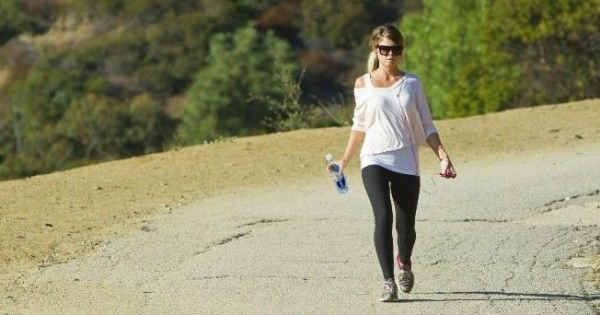
\includegraphics[width=0.4\textwidth]{figures/ssd1_coco}} \hspace{10pt}
	\subfigure[]{\includegraphics[width=0.4\textwidth]{figures/ssd1_voc}}
	\subfigure[]{\includegraphics[width=0.4\textwidth]{figures/ssd2_coco}} \hspace{10pt}
	\subfigure[]{\includegraphics[width=0.4\textwidth]{figures/ssd2_voc}}
	\subfigure[]{\includegraphics[width=0.4\textwidth]{figures/ssd3_coco}} \hspace{10pt}
	\subfigure[]{\includegraphics[width=0.4\textwidth]{figures/ssd3_voc}}
	\caption{Detección en distintas imágenes: (a)~Imagen sencilla con \acrshort{coco}, (b)~Imagen sencilla con \acrshort{voc}, (c)~Imagen complejo con \acrshort{coco}, (d)~Imagen compleja con \acrshort{voc}, (e)~Señal de tráfico con \acrshort{coco}, (f)~Señal de tráfico con \acrshort{voc}}
	\label{fig.ssd1}
\end{figure}

En una imagen bastante sencilla~(a) y~(b), el modelo de \textit{Pascal \acrshort{voc}} es capaz de detectar a la persona, mientras que el modelo \acrshort{coco} no la detecta. Por el contrario, en un escenario un poco más complicado~(c) y~(d), el modelo \acrshort{voc} no detecta uno de los coches de la escena, mientras que el modelo \acrshort{coco} realiza la detección de todos los coches. Por último, en las imágenes~(e) y~(f), la señal que aparece en primer plano queda identificada por \acrshort{coco}, pues entre sus etiquetas se incluyen este tipo de objetos, pero no por \acrshort{voc}, pues no incluyen etiquetas de este estilo.\\

Para tratar de obtener algún resultado concluyente se introdujo en la red una serie de imágenes de grises. Puesto que la red está entrenada con imágenes de color RGB será necesario replicar la propia imagen en las tres componentes para hacer coincidir las dimensiones de las imágenes y realizar la detección. En la Figura~\ref{fig.ssd2} se muestra cómo, con el modelo \acrshort{coco}~(a) y~(b), al realizar la detección en una imagen de grises, cuyo resultado en color era correcto para la persona a pesar de no detectar la bicicleta, comete un error a la hora de indicar la etiqueta de uno de los objetos detectados, equivocando la bicicleta con una persona. En el caso del modelo \acrshort{voc}~(c) y~(d) de la Figura~\ref{fig.ssd2}, se puede comprobar cómo se detecta un mayor número de personas al utilizar la imagen de grises que al emplear la imagen RGB.
\begin{figure}[H]
	\centering
	\subfigure[]{\includegraphics[width=0.4\textwidth]{figures/ssd4_color}} \hspace{10pt}
	\subfigure[]{\includegraphics[width=0.4\textwidth]{figures/ssd4_gris}}
	\subfigure[]{\includegraphics[width=0.4\textwidth]{figures/ssd5_color}} \hspace{10pt}
	\subfigure[]{\includegraphics[width=0.4\textwidth]{figures/ssd5_gris}}
	\caption{Detección en distintas imágenes: (a)~Imagen RGB con \acrshort{coco}, (b)~Imagen de grises con \acrshort{coco}, (c)~Imagen RGB con \acrshort{voc}, (d)~Imagen de grises con \acrshort{voc},}
	\label{fig.ssd2}
\end{figure}

Tras analizar las diferentes detecciones realizadas, tanto en imágenes RGB como de grises, no es posible establecer un resultado concluyente, pues no se observa una clara tendendia de mejora, estabilidad o empeoramiento de los resultados al variar las imágenes y los modelos utilizados. Además, la imágenes han sido escogidas de forma totalmente aleatoria, sin cumplir ningún tipo de característica que permita establecer conclusiones. Por todo ello, será necesario realizar un estudio más profundo de los modelos utilizados, con bases de datos de evaluación significativas, para obtener conclusiones sólidas sobre el enfoque \acrshort{ssd} de Caffe. \\


\lhead[]{CAPÍTULO \thechapter. CONCLUSIONES}
\chapter{Conclusiones y líneas futuras}\label{cap.conclusiones}
Por último, en este capítulo se exponen las conclusiones alcanzadas con el desarrollo del trabajo, así como posibles líneas para continuar en el futuro, ayudándose de los resultados obtenidos en el desarrollo del mismo.

\section{Conclusiones}
El desarrollo de este trabajo ha permitido establecer una serie de conclusiones en el ámbito de aprendizaje profundo mediante el empleo de redes neuronales entrenadas con Caffe. A pesar de que el desarrollo del trabajo tenía como objetivos establecer conclusiones sobre las dos tareas principales de esta técnica, clasificación y detección, por las propias características del trabajo únicamente se obtuvieron conclusiones firmes sobre la clasificación, dejando abierta la puerta a una futura investigación en el problema de la detección con estas redes. A continuación se exponen todas las conclusiones que fueron establecidas gracias a la obtención de distintos resultados por la evaluación de las redes neuronales entrenadas.

\begin{itemize}
	\item La plataforma Caffe posee un funcionamiento muy adecuado para el ámbito de la visión artificial gracias a un entrenamiento rápido y a gran número de ejemplos y facilidades para el mismo. Además proporcionan la posibilidad de entrenamiento de redes tanto para clasificación como detección.
	\item Las redes neuronales con Caffe pueden ser entrenadas con diferentes conjuntos de datos, siempre en formato \acrshort{lmdb}, obteniendo resultados muy diferentes en función de la composición de las mismas. 
	\item Para el ejemplo tratado con la base de datos \acrshort{mnist} para la clasificación de dígitos, al variar la composición de estas bases de datos, se han obtenido diversas conclusiones interesantes que han permitido mejorar de forma considerable la red final entrenada.
	\begin{itemize}
		\item El entrenamiento con imágenes de borde amplia el número aciertos en la clasificación, pues independiza la misma del fondo de la imagen.
		\item Al incluir imágenes con transformaciones en en entrenamiento de la red, la precisión de la clasificación aumenta, permitiendo obtener una red más robusta.
		\item La precisión obtenida al incluir un alto número de imágenes transformadas frente a la que se obtiene disminuyendo ese número de imágenes es muy similar, por lo que no es necesario incluir un gran número de estas imágenes en el entrenamiento.
		\item Sobre la inclusión de la imagen limpia en el entrenamiento, siendo ésta la imagen sin ninguna transformación, se obtienen resultados que avalan que no es necesario incluirla para obtener una mayor precisión.
	\end{itemize}
	\item Se ha elaborado un componente bastante y robusto con Python que permite la clasificación de dígitos mostrados a una cámara RGB gracias a una red entrenada con Caffe gracias a las conclusiones obtenidas en el punto anterior.
\end{itemize}

Como se mencionó anteriormente, los resultados obtenidos en los exprerimentos de la detección no son concluyenetes, por lo que no es posible establecer conclusiones firmes sobre esta técnica.

\section{Líneas futuras}
Para seguir con la investigación abordada en este trabajo se pueden seguir dos claras tendencias marcadas por los dos grande problemas que se pueden abordar, detección y clasificación.
\begin{itemize}
	\item Por un lado, el que no se haya obtenido resultados concluyentes en el campo de la detección permite continuar en futuras investigaciones en esta línea, tratando de obtener una red robusta para esta tarea mediante la modificación de la red entrenada con diferentes bases de datos o estructuras de red.
	\item Por otro lado, en el campo de la clasificación, es posible extender lo aprendido para un ejemplo sencillo, la clasificación de dígitos con redes neuronales gracias al conjunto de datos \acrshort{mnist}, a un ejemplo más complejo como puede ser la clasificación de signos o de señales de tráfico.
\end{itemize}

Finalmente, la aplicación ideal consiste en una mezcla de ambos problemas. De esta manera, por ejemplo, sería posible la elaboración de una aplicación que permitiese a un choche circular de forma autónoma, detectando los estímulos que recibe de la carretera y clasificando los mismos para actuar en consecuencia a la clase detectada.\\

Éstos son solo algunos ejemplos de los diferentes problemas que se pueden tratar de abordar con esta tecnología. La cantidad de tareas que se pueden tratar de realizar es tan amplia como el número de problemas que se le pueden presentar a un ser humano en su día a día, pues la finalidad de estas aplicaciones no es otra que facilitar la vida diaria de las personas.

%%%%%%%%%%%%%%% Bibliograí­a %%%%%%%%%%%%%%%
\lhead[]{BIBLIOGRAFÍA}
\addcontentsline{toc}{chapter}{Bibliografía}
\bibliographystyle{unsrt}
\bibliography{Memoria}

\end{document}